% Festlegung des Allgemeinen Dokumentenformats
\documentclass[a4paper,12pt,headsepline,parskip]{scrartcl}

% Umlaute unter UTF8 nutzen
\usepackage[utf8]{inputenc}

% Variablen
%Variablen welche innerhalb der gesamten Arbeit zur Verfügung stehen sollen
\newcommand{\titleDocument}{Projekt Programmierung}
\newcommand{\subjectDocument}{im Studiengang <Studiengang>}
\newcommand{\Matrikelnummer}{50855}
\newcommand{\Thema}{Entwicklung eines Anwesenheitsplaners für das SMK}
\newcommand{\Abgabedatum}{19.07.2023}
\newcommand{\Studiengang}{Informatik}



%Tabellen
%\usepackage{tabularray}
%\usepackage{makecell}
%\usepackage{array}
%\usepackage{ragged2e}
%\usepackage{multirow}
%\usepackage{rotating}

%Code
\usepackage{listings}

%Schriftart
\usepackage{helvet}
\renewcommand\familydefault{\sfdefault}

% weitere Pakete
% Grafiken aus PNG Dateien einbinden
\usepackage{graphicx}


% Deutsche Sonderzeichen und Silbentrennung nutzen
\usepackage[ngerman]{babel}

% Eurozeichen einbinden
\usepackage[right]{eurosym}

% Zeichenencoding
\usepackage[T1]{fontenc}

\usepackage{lmodern}

% floatende Bilder ermöglichen
%\usepackage{floatflt}

% mehrseitige Tabellen ermöglichen
\usepackage{longtable}

% Unterstützung für Schriftarten
%\newcommand{\changefont}[3]{ 
%\fontfamily{#1} \fontseries{#2} \fontshape{#3} \selectfont}

% Packet für Seitenrandabständex und Einstellung für Seitenränder
\usepackage{geometry}
\geometry{left=2.5cm, right=1.5cm, top=2.5cm, bottom=2cm}

% Paket für Boxen im Text
\usepackage{fancybox}

% bricht lange URLs "schön" um
\usepackage[hyphens,obeyspaces,spaces]{url}

% Paket für Textfarben
\usepackage{color}

% Mathematische Symbole importieren
\usepackage{amssymb}

% auf jeder Seite eine Überschrift (alt, zentriert)
%\pagestyle{headings}

% erzeugt Inhaltsverzeichnis mit Querverweisen zu den Abschnitten (PDF Version)
\usepackage[bookmarksnumbered,pdftitle={\titleDocument},hyperfootnotes=false]{hyperref}
%\hypersetup{colorlinks, citecolor=red, linkcolor=blue, urlcolor=black}
%\hypersetup{colorlinks, citecolor=black, linkcolor= black, urlcolor=black}

% neue Kopfzeilen mit fancypaket
\usepackage{fancyhdr} %Paket laden
\pagestyle{fancy} %eigener Seitenstil
\fancyhf{} %alle Kopf- und Fußzeilenfelder bereinigen
\fancyhead[L]{\nouppercase{\leftmark}} %Kopfzeile links
\fancyhead[C]{} %zentrierte Kopfzeile
\fancyhead[R]{\thepage} %Kopfzeile rechts
\renewcommand{\headrulewidth}{0.4pt} %obere Trennlinie
%\fancyfoot[C]{\thepage} %Seitennummer
%\renewcommand{\footrulewidth}{0.4pt} %untere Trennlinie

% für Tabellen
\usepackage{array}

% Runde Klammern für Zitate
%\usepackage[numbers,round]{natbib}

% Festlegung Art der Zitierung - Havardmethode: Abkuerzung Autor + Jahr
\bibliographystyle{alphadin}

% Schaltet den zusätzlichen Zwischenraum ab, den LaTeX normalerweise nach einem Satzzeichen einfügt.
%\frenchspacing

\usepackage{xspace} % sorgt dafür, dass Leerzeichen hinter parameterlosen Makros nicht als Makroendezeichen interpretiert werden

% Paket für Zeilenabstand
\usepackage{setspace}

% für Bildbezeichner
\usepackage{capt-of}

% für Stichwortverzeichnis
\usepackage{makeidx}

%Konfiguriere das Inhaltsverzeichnis
\usepackage{tocbasic}
\DeclareTOCStyleEntries[
  raggedentrytext,
  numwidth=0pt,
  numsep=1ex,
  dynnumwidth,
]{tocline}{chapter,section,subsection,subsubsection,paragraph,subparagraph}
\DeclareTOCStyleEntries[
  indent=0pt,
  linefill=\TOCLineLeaderFill,
]{tocline}{section,subsection,subsubsection,paragraph,subparagraph}
\DeclareTOCStyleEntries[
  indent=10pt,
]{tocline}{subsection,subsubsection,paragraph,subparagraph}

% für Listings
\usepackage{listings}
\lstset{numbers=left, numberstyle=\tiny, numbersep=5pt, keywordstyle=\color{black}\bfseries, stringstyle=\ttfamily,showstringspaces=false,basicstyle=\footnotesize,captionpos=b}
\lstset{language=csh}

% Indexerstellung
\makeindex

% Abkürzungsverzeichnis
%\usepackage[german]{nomencl}
%\let\abbrev\nomenclature

% Abkürzungsverzeichnis LiveTex Version
% Titel des Abkürzungsverzeichnisses
%\renewcommand{\nomname}{Codesegmente}
% Abstand zwischen Abkürzung und Erläuterung
%\setlength{\nomlabelwidth}{.25\textwidth}
% Zwischenraum zwischen Abkürzung und Erläuterung mit Punkten
%\renewcommand{\nomlabel}[1]{#1 \dotfill}
% Variation des Abstandes der einzelnen Abkürzungen zu einander
%\setlength{\nomitemsep}{-\parsep}
% Index mit Abkürzungen erzeugen
%\makenomenclature
%\makeglossary

% Abkürzungsverzeichnis TeTEX Version
% \usepackage[german]{nomencl}
% \makenomenclature
% %\makeglossary
% \renewcommand{\nomname}{Abkürzungsverzeichnis}
% \AtBeginDocument{\setlength{\nomlabelwidth}{.25\columnwidth}}
% \renewcommand{\nomlabel}[1]{#1 \dotfill}
% \setlength{\nomitemsep}{-\parsep}

% Optional: Einzelne Zeilen am Anfang einer Seite unterdrücken (Schusterjungen)
% \clubpenalty = 10000
% Optional: Einzelne Zeilen am Ende einer Seite unterdrücken (Hurenkinder)
% \widowpenalty = 10000
% \displaywidowpenalty = 10000

\begin{document}
% hier werden die Trennvorschläge inkludiert
%hier müssen alle Wörter rein, welche Latex von sich auch nicht korrekt trennt bzw. bei denen man die genaue Trennung vorgeben möchte
\hyphenation{
Film-pro-du-zen-ten
Lux-em-burg
Soft-ware-bau-steins
zeit-in-ten-siv
}


%Befehle
% !TEX root = ../Projektdokumentation.tex


% Abkürzungen, ggfs. mit korrektem Leerraum
\newcommand{\bs}{$\backslash$\xspace}
\newcommand{\bspw}{bspw.\xspace}
\newcommand{\bzw}{bzw.\xspace}
\newcommand{\ca}{ca.\xspace}
\newcommand{\dahe}{\mbox{d.\,h.}\xspace}
\newcommand{\etc}{etc.\xspace}
\newcommand{\eur}[1]{\mbox{#1\,\texteuro}\xspace}
\newcommand{\evtl}{evtl.\xspace}
\newcommand{\ggfs}{ggfs.\xspace}
\newcommand{\Ggfs}{Ggfs.\xspace}
\newcommand{\gqq}[1]{\glqq{}#1\grqq{}}
\newcommand{\inkl}{inkl.\xspace}
\newcommand{\insb}{insb.\xspace}
\newcommand{\ua}{\mbox{u.\,a.}\xspace}
\newcommand{\usw}{usw.\xspace}
\newcommand{\Vgl}{Vgl.\xspace}
\newcommand{\zB}{\mbox{z.\,B.}\xspace}

% Befehle für häufig anfallende Aufgaben
\newcommand{\Abbildung}[1]{\autoref{fig:#1}}
\newcommand{\Anhang}[1]{\appendixname{}~\ref{#1}: \nameref{#1} \vpageref{#1}}
\newcommand{\Sektion}[1]{\ref{#1}: \nameref{#1} \vpageref{#1}}
\newcommand{\includegraphicsKeepAspectRatio}[2]{\includegraphics[width=#2\textwidth,height=#2\textheight,keepaspectratio]{#1}}
\newcommand{\Zitat}[2][\empty]{\ifthenelse{\equal{#1}{\empty}}{\citep{#2}}{\citep[#1]{#2}}}
\newcommand{\Autor}[1]{\textsc{#1}} % zum Ausgeben von Autoren
\newcommand{\itemd}[2]{\item{\textbf{#1}}\\{#2}} % erzeugt ein Listenelement mit fetter Überschrift

% fügt Tabellen aus einer TEX-Datei ein
\newcommand{\tabelle}[3] % Parameter: caption, label, file
{\begin{table}[htbp]
    \centering
    \singlespacing
    \input{Tabellen/#3}
    \caption{#1}
    \label{#2}
  \end{table}}

\newcommand{\tabelleAnhang}[1] % Parameter: file
{\begin{center}
    \singlespacing
    \input{Tabellen/#1}
  \end{center}}

% einfaches Wechseln der Schrift, z.B.: \changefont{cmss}{sbc}{n}
\newcommand{\changefont}[3]{\fontfamily{#1} \fontseries{#2} \fontshape{#3} \selectfont}

% Verwendung analog zu \includegraphics
\newlength{\myx} % Variable zum Speichern der Bildbreite
\newlength{\myy} % Variable zum Speichern der Bildhöhe
\newcommand\includegraphicstotab[2][\relax]{%
  % Abspeichern der Bildabmessungen
  \settowidth{\myx}{\includegraphics[{#1}]{#2}}%
  \settoheight{\myy}{\includegraphics[{#1}]{#2}}%
  % das eigentliche Einfügen
  \parbox[c][1.1\myy][c]{\myx}{%
    \includegraphics[{#1}]{#2}}%
}

\definecolor{AOBlau}{rgb}{0, 0.28, 0.56}

% verschiedene Befehle um Wörter semantisch auszuzeichnen ----------------------
\newcommand{\Index}[2][\empty]{\ifthenelse{\equal{#1}{\empty}}{\index{#2}#2}{\index{#1}#2}}
\newcommand{\Fachbegriff}[2][\empty]{\ifthenelse{\equal{#1}{\empty}}{\textit{\Index{#2}}}{\textit{\Index[#1]{#2}}}}
\newcommand{\NeuerBegriff}[2][\empty]{\ifthenelse{\equal{#1}{\empty}}{\textbf{\Index{#2}}}{\textbf{\Index[#1]{#2}}}}

\newcommand{\Ausgabe}[1]{\texttt{#1}}
\newcommand{\Eingabe}[1]{\texttt{#1}}
\newcommand{\Code}[1]{\texttt{#1}}
\newcommand{\Datei}[1]{\texttt{#1}}

\newcommand{\Assembly}[1]{\textsf{#1}}
\newcommand{\Klasse}[1]{\textsf{#1}}
\newcommand{\Methode}[1]{\textsf{#1}}
\newcommand{\Attribut}[1]{\textsf{#1}}

\newcommand{\Datentyp}[1]{\textsf{#1}}
\newcommand{\XMLElement}[1]{\textsf{#1}}
\newcommand{\Webservice}[1]{\textsf{#1}}

\newcommand{\Refactoring}[1]{\Fachbegriff{#1}}
\newcommand{\CodeSmell}[1]{\Fachbegriff{#1}}
\newcommand{\Metrik}[1]{\Fachbegriff{#1}}
\newcommand{\DesignPattern}[1]{\Fachbegriff{#1}}


% Schriftart Helvetica verwenden



% Leere Seite am Anfang
\thispagestyle{empty} % erzeugt Seite ohne Kopf- / Fusszeile
\mbox{}
\newpage

% Titelseite %
\thispagestyle{empty}


\begin{figure}[t]
 \centering
 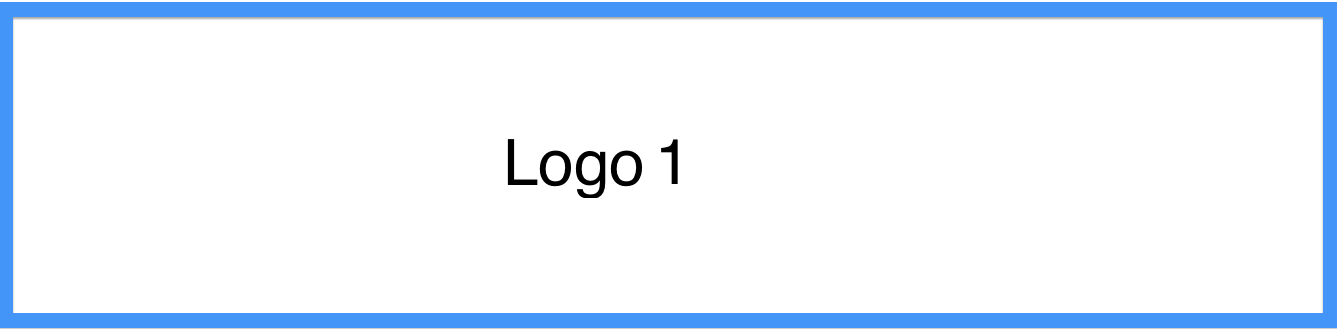
\includegraphics[width=0.6\textwidth]{abb/logo1}
~~~~~~~~~~
 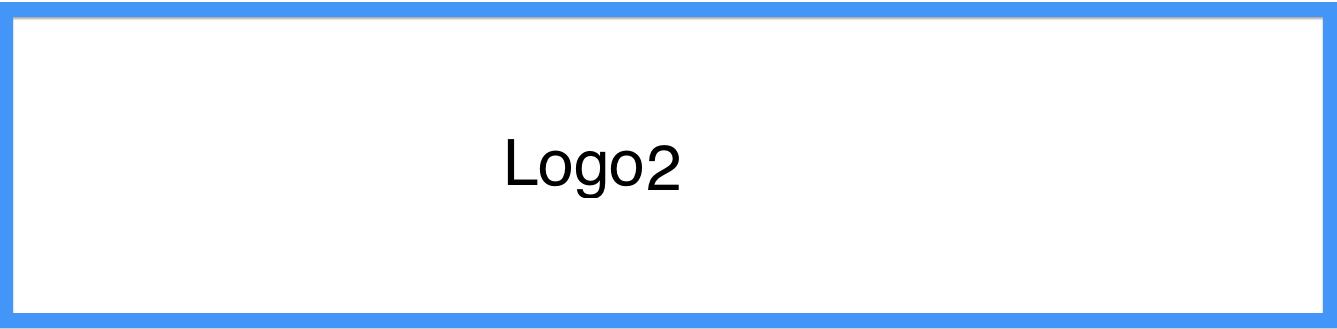
\includegraphics[width=0.3\textwidth]{abb/logo2}
\end{figure}


\begin{verbatim}


\end{verbatim}

\begin{center}
\Large{Fachhochschule <Name>}\\
\Large{- Campus <Name> -}\\
\end{center}


\begin{center}
\Large{Fakultät für <Fachrichtung>}
\end{center}
\begin{verbatim}




\end{verbatim}
\begin{center}
\doublespacing
\textbf{\LARGE{\titleDocument}}\\
\singlespacing
\begin{verbatim}

\end{verbatim}
\textbf{{~\subjectDocument~-~Schwerpunkt <Schwerpunktfach>}}
\end{center}
\begin{verbatim}

\end{verbatim}
\begin{center}

\end{center}
\begin{verbatim}

\end{verbatim}
\begin{center}
\textbf{zur Erlangung des akademischen Grades \\ Bachelor / Master of Science}
\end{center}
\begin{verbatim}






\end{verbatim}
\begin{flushleft}
\begin{tabular}{llll}
\textbf{Thema:} & & <Thema der Arbeit> & \\
& & \\
\textbf{Autor:} & & Name <name@mail.de>& \\
& & MatNr. 12345... & \\
& & \\
\textbf{Version vom:} & & \today &\\
& & \\
\textbf{1. Betreuerin:} & & Prof. Dr. X &\\
\textbf{2. Betreuer:} & & Prof. Dr. Y &\\
\end{tabular}
\end{flushleft}


% römische Numerierung
\pagenumbering{roman}

% 1.5 facher Zeilenabstand
\onehalfspacing

\newpage

% Sperrvermerk
%\thispagestyle{empty}
%\section*{Sperrvermerk}
\textcolor{red}{
Die vorliegende Arbeit beinhaltet interne und vertrauliche Informationen der Firma <Firmenname>.
Die Weitergabe des Inhalts der Arbeit im Gesamten oder in Teilen sowie das Anfertigen
von Kopien oder Abschriften - auch in digitaler Form - sind grundsätzlich untersagt.
Ausnahmen bedürfen der schriftlichen Genehmigung der Firma <Firmenname>.
}


% Eidesstattliche Erklärung
\newpage
\phantomsection
\addcontentsline{toc}{section}{Eidesstattliche Erklärung}
\section*{Selbstständigkeitserklärung }
\thispagestyle{empty}

\begin{verbatim}

\end{verbatim}

\begin{LARGE}Erklärung zur selbstständigen Anfertigung der Arbeit \end{LARGE}
\begin{verbatim}


\end{verbatim}
Ich versichere, dass ich die Arbeit selbstständig angefertigt und keine anderen als die angegebenen Hilfsmittel benutzt habe. Wörtlich oder sinngemäß aus anderen Quellen übernommene Textstellen, Bilder, Tabellen u. a. sind unter Angabe der Herkunft kenntlich gemacht. Weiterhin versichere ich, dass diese Arbeit oder eine ähnliche Arbeit mit in Teilen wesentlicher Inhaltsübereinstimmung noch keiner anderen Prüfungsbehörde vorgelegt wurde.





\begin{flushleft}Dresden, am 19.07.2023:\end{flushleft} 
\begin{flushright}Martin Lee Starke\end{flushright}




\newpage

% Einleitung / Abstract
%\thispagestyle{empty}
%\section*{Zusammenfassung}

Hier steht der Text, welcher den Inhalte der Arbeit zusammenfasst...

Lorem ipsum dolor sit amet, consetetur sadipscing elitr, sed diam nonumy eirmod tempor invidunt ut labore et dolore magna aliquyam erat, sed diam voluptua. At vero eos et accusam et justo duo dolores et ea rebum. Stet clita kasd gubergren, no sea takimata sanctus est Lorem ipsum dolor sit amet. Lorem ipsum dolor sit amet, consetetur sadipscing elitr, sed diam nonumy eirmod tempor invidunt ut labore et dolore magna aliquyam erat, sed diam voluptua. At vero eos et accusam et justo duo dolores et ea rebum. Stet clita kasd gubergren, no sea takimata sanctus est Lorem ipsum dolor sit amet.

\section*{Abstract}

Here goes the English text which summarizes the content of the thesis...

Lorem ipsum dolor sit amet, consetetur sadipscing elitr, sed diam nonumy eirmod tempor invidunt ut labore et dolore magna aliquyam erat, sed diam voluptua. At vero eos et accusam et justo duo dolores et ea rebum. Stet clita kasd gubergren, no sea takimata sanctus est Lorem ipsum dolor sit amet. Lorem ipsum dolor sit amet, consetetur sadipscing elitr, sed diam nonumy eirmod tempor invidunt ut labore et dolore magna aliquyam erat, sed diam voluptua. At vero eos et accusam et justo duo dolores et ea rebum. Stet clita kasd gubergren, no sea takimata sanctus est Lorem ipsum dolor sit amet.


% einfacher Zeilenabstand
\singlespacing

\newpage
% Seitenzählung bei Inhaltsverzeichnis beginnen
\setcounter{page}{1}

% Inhaltsverzeichnis anzeigen
\thispagestyle{empty}
\tableofcontents

\newpage
% das Abbildungsverzeichnis
% Verion 1: Abbildungsverzeichnis MIT führender Nummberierung endgueltig anzeigen
\listoffigures
% Abbildungsverzeichnis soll im Inhaltsverzeichnis auftauchen
\addcontentsline{toc}{section}{Abbildungsverzeichnis}

% Verion 2: Abbildungsverzeichnis OHNE führende Nummberierung endgueltig anzeigen
%\begingroup
%\renewcommand\numberline[1]{}
%\listoffigures
%\endgroup


% das Tabellenverzeichnis
\newpage
% \fancyhead[L]{Abbildungsverzeichnis / Abkürzungsverzeichnis} %Kopfzeile links
% Tabellenverzeichnis endgültig anzeigen
\listoftables
% Tabellenverzeichnis soll im Inhaltsverzeichnis auftauchen
\addcontentsline{toc}{section}{Tabellenverzeichnis}

%% WORKAROUND für Listings
%\makeatletter% --> De-TeX-FAQ
%\renewcommand*{\lstlistoflistings}{%
%  \begingroup
%    \if@twocolumn
%      \@restonecoltrue\onecolumn
%    \else
%      \@restonecolfalse
%    \fi
%    \lol@heading
%    \setlength{\parskip}{\z@}%
%    \setlength{\parindent}{\z@}%
%    \setlength{\parfillskip}{\z@ \@plus 1fil}%
%    \@starttoc{lol}%
%    \if@restonecol\twocolumn\fi
%  \endgroup
%}
%\makeatother% --> \makeatletter
% das Listingverzeichnis
\newpage
\fancyhead[L]{Listingverzeichnis} %Kopfzeile links
\renewcommand{\lstlistlistingname}{Listingverzeichnis}
\lstlistoflistings
% Listingverzeichnis soll im Inhaltsverzeichnis auftauchen
\addcontentsline{toc}{section}{Listingverzeichnis}
%%%%

% das Abkürzungsverzeichnis
%\newpage
% das Abkürzungsverzeichnis ausgeben
%\fancyhead[L]{Abkürzungsverzeichnis} %Kopfzeile links
%\nomenclature{UGC}{User Generated Content}
\nomenclature{CSS}{Cascading Style Sheets}
\nomenclature{JS}{JavaScript}
\nomenclature{SQL}{Structured Query Language}
\nomenclature{GPL}{GNU General Public License}
\nomenclature{GNU}{GNU is not Unix}
\nomenclature{LGPL}{GNU Lesser General Public License}
\nomenclature{XMPP}{Extensible Messaging and Presence Protocol}
\nomenclature{IM}{Instant Message}
\nomenclature{CMS}{Content Management System}
\nomenclature{RSS}{Really Simple Syndication}
\nomenclature{JSON}{JavaScript Object Notation}
\nomenclature{HTML}{Hypertext Markup Language}
\nomenclature{TDD}{Test-driven development}
\nomenclature{GUI}{Graphical User Interface}
\nomenclature{KPI}{Key Performance Indicator}
\nomenclature{WWW}{World Wide Web}
\nomenclature{OCR}{Optical Character Recognition}
\nomenclature{ERM}{Entity Relationship Modell}

%\printnomenclature[3cm]
% Abkürzungsverzeichnis soll im Inhaltsverzeichnis auftauchen
%\addcontentsline{toc}{section}{Abkürzungsverzeichnis}


%%%%%%% EINLEITUNG %%%%%%%%%%%%
\newpage
\fancyhead[L]{\nouppercase{\leftmark}} %Kopfzeile links

% 1,5 facher Zeilenabstand
\onehalfspacing

% arabische Seitennummerierung ab hier
\pagenumbering{arabic}

% Alternative Einbindung des Abstract in Kapitel "0" falls gewünscht
%\setcounter{section}{-1}
%\setcounter{page}{0}

% Option: Einbindung abstract
%\section*{Zusammenfassung}

Hier steht der Text, welcher den Inhalte der Arbeit zusammenfasst...

Lorem ipsum dolor sit amet, consetetur sadipscing elitr, sed diam nonumy eirmod tempor invidunt ut labore et dolore magna aliquyam erat, sed diam voluptua. At vero eos et accusam et justo duo dolores et ea rebum. Stet clita kasd gubergren, no sea takimata sanctus est Lorem ipsum dolor sit amet. Lorem ipsum dolor sit amet, consetetur sadipscing elitr, sed diam nonumy eirmod tempor invidunt ut labore et dolore magna aliquyam erat, sed diam voluptua. At vero eos et accusam et justo duo dolores et ea rebum. Stet clita kasd gubergren, no sea takimata sanctus est Lorem ipsum dolor sit amet.

\section*{Abstract}

Here goes the English text which summarizes the content of the thesis...

Lorem ipsum dolor sit amet, consetetur sadipscing elitr, sed diam nonumy eirmod tempor invidunt ut labore et dolore magna aliquyam erat, sed diam voluptua. At vero eos et accusam et justo duo dolores et ea rebum. Stet clita kasd gubergren, no sea takimata sanctus est Lorem ipsum dolor sit amet. Lorem ipsum dolor sit amet, consetetur sadipscing elitr, sed diam nonumy eirmod tempor invidunt ut labore et dolore magna aliquyam erat, sed diam voluptua. At vero eos et accusam et justo duo dolores et ea rebum. Stet clita kasd gubergren, no sea takimata sanctus est Lorem ipsum dolor sit amet.

%\newpage

% einzelne Kapitel werden hier eingebunden
\section{Einleitung}
\label{sec:Einleitung}
Diese Arbeit beschäftigt sich mit der Umsetzung eines Softwareprojektes im Zuge des Modules Programmierung Projekt Sommersemester 2023. Dabei soll ein selbstgewähltes Softwareentwicklungsprojekt umgesetzt und mit einer wissenschaftlichen Arbeit dokumentiert werden. In dieser Arbeit werden alle Projektphasen der Umsetzung des Projektes beleuchtet, wobei der Fokus auf den konzeptionellen Teilen liegt. Nach der Abhandlung der einzelnen Projektphasen soll die entwickelte Software als Ergebnis der Arbeit mit ihrem Funktionsumfang und den wichtigsten Codeelementen vorgestellt werden.

\subsection{Projektumfeld}
\label{sec:Projektumfeld}
Der Praxispartner für dieses Projekt ist das Sächsische Staatsministerium für Kultus (SMK). Das SMK ist ein Ministerium der Landesregierung und fungiert als oberste Schulaufsichtsbehörde im Freistaat Sachsen. Damit ist das SMK für die Umsetzung der Bildungspolitik zuständig. Zu den Hauptaufgaben zählen vor allen Dingen die Planung und Verwaltung von Schulen und Kindertageseinrichtungen, insbesondere das Festlegen von Richtlinien und die Ausarbeitung von Lehrplänen.

Das SMK ist in vier Abteilungen mit jeweils mehreren Fachreferaten unterteilt siehe \ref{abb:Organigramm}. Zusätzlich gehört das Landesamt für Schule und Bildung (LaSuB), mit mehreren Standorten in ganz Sachsen zum nachgeordneten Bereich des SMK. Insgesamt trägt das SMK sorge für über 38.000 Beschäftigte und mehr als 685.000 Kinder und Jugendliche in sächsischen Kindertageseinrichtungen und Schulen.

Im Hauptgebäude am Carolaplatz 1 arbeiten ca. 250 Bedienstete die sich auf fünf Etagen verteilen. Das führt dazu, dass die Verfügbarkeit von Mitarbeitern für Kollegen und Referatsleiter nicht unmittelbar ersichtlich ist. Deswegen endstand in jedem Referat je nach Bedarf eine eigene Anwesenheitsliste in unterschiedlichen Ausprägungen. Die Komplexität und Nutzungsfrequenz dieser Listen stieg im Laufe der letzten Jahre stetig an, da die Arbeit von Zuhause aus und mobiles Arbeiten immer weiter in den Arbeitsalltag integriert wurden. Das führte letztlich zu einigen Problemen die mit der Entwicklung eines einheitlichen Anwesenheitsplaners für alle Referate behoben werden sollen.

Die Umsetzung des Projektes erfolgt dabei durch Referat 12 und in enger Zusammenarbeit mit Referat 22 und den Datenschutzbeauftragen sowie des Informationssicherheitsbeauftragten des SMK. Als Projektleiter ist die zuständige IT-Referentin aus Referat 12 eingesetzt.

\subsection{Projektmotivation}
\label{sec:Projektmotivation}
Das Projekt zielt darauf ab, eine neue Lösung für die Anwesenheitsplanung zu finden. Derzeit erfolgt die Planung von Anwesenheiten der Bediensteten der jeweiligen Referate mithilfe von Excel-Dateien. Dieser Ansatz stößt jedoch auf verschiedene Probleme, die dringend angegangen werden müssen.

Das Hauptproblem besteht darin, dass die Funktionsweise von MS Excel in der für den Freistaat Sachsen verfügbaren Version nicht zulässt, ein Dokument parallel durch zwei Nutzer zu öffnen \bzw zu bearbeiten. Dies führt zu häufigen Fehlermeldungen, wenn ein Bediensteter das Dokument bereits geöffnet hat und ein zweiter parallel darauf zugreifen möchte. Infolgedessen kommt es zu Frustration bei den Mitarbeitern und Fehlern in der Anwesenheitsplanung. Die Fehlerbehebung muss oft vom IT-Referat bewältigt werden und erzeugt dadurch zusätzlichen Arbeitsaufwand.

Ein weiterer wichtiger Aspekt ist der zunehmende Bedarf an Planungsmöglichkeiten der Anwesenheiten der Mitarbeiter aufgrund der vermehrten Nutzung von Homeoffice. In der heutigen Arbeitswelt ist es für viele Unternehmen und Organisationen üblich geworden, ihren Mitarbeitern die Möglichkeit zu geben, von zu Hause aus oder mobil zu arbeiten. Dies sorgt jedoch auch für neue Herausforderungen bei der Anwesenheitsplanung. Es ist entscheidend, dass sowohl die Referatsleiter als auch die Bediensteten einen klaren Überblick über die lokale Anwesenheit ihrer Kollegen haben, um vor Ort Tätigkeiten abzustimmen und \zB Funktionszeiten zu gewährleisten.

Angesichts dieser Probleme und Anforderungen besteht ein dringender Bedarf an einer soliden Lösung für die Anwesenheitsplanung. Eine solche Lösung sollte es den Benutzern ermöglichen, gleichzeitig auf die Anwesenheitsliste zuzugreifen und diese zu bearbeiten. Darüber hinaus sollte das Format benutzerfreundlich sein und den Referatsleitern und Bediensteten den Überblick über die Anwesenheit der Mitarbeiter erleichtern.


\subsection{Projektziel}
\label{sec:Projektziel}

Das Ziel dieses Projektes ist es, eine effiziente und benutzerfreundliche Lösung für die Anwesenheitsplanung zu entwickeln und allen Referaten zentral bereitzustellen. Dafür soll eine geeignete Softwarelösung geschaffen und implementiert werden, welche die Einschränkungen der Excel-Datei behebt und möglichst viele Anforderungen für die Anwesenheitsplanung aus den Referaten erfüllt. Zu beachten sind hierbei die Datenschutz- und Datensicherheitsanforderung auf Grundlage der Informationssicherheitsrichtlinien des SMK.

\subsection{Projektplanung}
\label{sec:Projektplanung}

Eine gründliche Projektplanung ist essenziell für ein Softwareentwicklungsprojekt um einen strukturierten und effizienten Ablauf zu gewährleisten. Für die Ablaufplanung kann auf das Grundmodell des Projektmanagements nach \cite[S.225]{dehler-2013} zurückgegriffen werden. Demnach besteht ein Projekt aus Analyse-, Entwurfs-, Implementierungs- und Testphase. Für die Entwicklung wird das Wasserfallmodell als standardisiertes Softwareentwicklungsverfahren verwendet, da das umzusetzende Projekt nur über einen kleinen zeitlichen Rahmen verfügt und überschaubar komplex ist.

%TODO: Wasserfallmodell als Quelle aus Buch!
Für eine bessere Übersicht des Projektablaufs wurde ein Gantt Diagramm für die Zeitplanung mit Meilensteinen erstellt, siehe Anhang \ref{abb:Gantt}. Für die Umsetzung des Projektes nimmt die Analysephase mit der Ist- und Soll-Analyse eine besonders wichtige Positionen ein. In der Ist-Analyse werden die bestehenden Anwesenheitsplanungsmethoden der Referate und deren Schwachstellen untersucht. Der Soll-Zustand wird durch eine Anforderungsanalyse ermittelt, um die Anforderungen und Ziele des Projekts klar zu definieren. Hierbei sollen sowohl von Mitarbeitern, als auch durch die Analyse der vorhandenen Datenbestände in den Anwesenheitslisten gewonnene Informationen ausgewertet werden um relevante Anforderungen zu identifizieren. Diese Anforderungen dienen als Grundlage für die Design- und Implementierungsphase, in der die eigentliche Entwicklung der Software stattfindet.

Nach Abschluss der Implementierung soll ein lauffähiger Prototyp entstehen, der dann für Tests verwendet werden kann. Sobald die Testphase erfolgreich abgeschlossen ist, kann die Software in die Produktivumgebung migriert werden. Dieser Prozess bildet den Abschluss des Projektes.



\section{Analysephase}
\label{sec:Analysephase}
%TODO:Quelle Recherche Problemdefinition / Requiremants Engeneering
Die Analysephase eines Softwareentwicklungsprojekts spielt eine entscheidende Rolle für den Erfolg eines Projekts, da hier die Anforderungen an das zu entwickelnde System erhoben werden. Zur Ermittlung der Anforderungen soll eine Systemanalyse und eine Anforderungsanalyse durchgeführt werden, die Einblicke in die bisherigen Prozesse der Anwesenheitsplanung geben sollen. Für die Informationsbeschaffung soll auf die Analysemethode der Datenanalyse gesetzt werden. Um die so gewonnenen Daten zu Validieren und auch subjektive Verbesserungsvorschläge zu berücksichtigen werden ebenfalls Intervierws mit den Mitarbeitern durchgeführt. Die dabei erhobenen Daten werden dann Aufbereitet und Modelliert.

In den folgenden Abschnitte beschreiben die Vorgehensweise und Ergebnisse der durchgeführten Analysen. Die dabei gewonnenen Erkenntnisse bilden die grundlage für die weiteren Entscheidungen für die Umsetzung des Projektes.


\subsection{Analyse des Ist-Zustandes}
\label{sec:Ist-Zustand}

%TODO:Bestehende Anwesenheitsplanungsmethoden (Intervierws mit Mitarbeitern + Analyse der Exeldateien)
%TODO:Schwachstellen und Herausforderungen im aktuellen Prozess (Recht,keine Intigrität,kein mehrfacher zugriff,nur ecxel zugreifbar)

% Bestehende Anwesenheitsplanungsmethoden (Datenstruktur/Tabellenaufbau)
% Schwachstellen und Herausforderungen im aktuellen Prozess
Um eine verbesserte Variante eines Anwesenheitsplaners zu erstellen ist es notwendig die bestehenden Systeme und Abläufe zu verstehen. Dafür wurden Interviews mit Mitarbeitern aus verschiedenen Referaten geführt und analog dazu die verschiedenen Excel-Dateien analysiert. Dabei lag der Fokus auf der Analyse des Prozesses der Anwesenheitsplanung, um diesen durch die neue Variante des Anwesenheitsplaners bestmöglich zu unterstützen. 

Die Interviews ergaben, dass das Excel-Dokument meist in einem Netzlaufwerk aufbewahrt wird um für die Rederatsmitglieder zugänglich zu sein. Das Dokument wird nicht anders behandelt als andere Referatsdaten was bedeutet, dass es keine spezielle Rechteverwaltung gibt. Das führt zu Fehler und Inkonsistenzen durch versehentliches ändern anderer Datensätze, da schreibrechte auf das ganze Dokument vergeben sind.

Als größte Problem wurde die Tatsache, dass nur ein Nutzer gleichzeitig auf das Excel-Dokument zugreifen kann festgestellt. Dies führt dazu, dass für eine unbestimmte Zeit keine Möglichkeit besteht den eigenen Status zu ändern. Meistens tritt der Umstand auf, wenn ein Mitarbeiter die Datei im Hintergrund geöffnet hat diese aber nicht nutzt.   

Für die Datenanalyse wurden von den beteiligten Referaten eine Kopie ihrer Excel Datei zur Verfügung gestellt. Hauptsächlich sollte der grafische Aufbau der Tabelle und die enthaltenen Informationen der Tabellen untersucht werden. Die Analyse ergab, dass alle Anwesenheitsplaner Tabellen ähnlich aufgebaut sind. Unterschiede ergaben sich meist nur in der Bezeichnung der Anwesenheitszustände und die Granularität der Zeitabschnitte. Um eine Referenz für die weitere Entwicklung zu haben wurde aus den Referats-Tabellen eine Modelltabelle für die Anwesenheitsplanung erstellt.
%Basierend auf diesen Erkenntnissen wird deutlich, dass eine dringende Notwendigkeit besteht, den Anwesenheitsplaner zu verbessern. Eine effektive Lösung sollte die Möglichkeit bieten, dass mehrere Nutzer gleichzeitig auf die Anwesenheitsdaten zugreifen und diese aktualisieren können. Die Automatisierung von Prozessen und die Integration einer Datenbank könnten die Genauigkeit, Effizienz und Benutzerfreundlichkeit des Anwesenheitsplaners erheblich verbessern.

\subsection{Anforderungen an den Anwesenheitsplaner}
\label{sec:Soll-Zustand}
%TODO:UseCase
%TODO:Kernfunktionen
%TODO:Umsetzungsrichtlinien
%TODO:Berechtigungensonzept

\subsection{ Datenschutz und Datensicherheitsanalyse}
\label{sec:Datenschutz}
%TODO:Personenbezogene Daten?
%TODO:Anforderungen Datenschutzkonzept
%TODO:Datensicherheit / Risikoanalyse
\section{Variantendiskussion}
\label{sec:Variantendiskussion}
Zu Beginn soll eine Marktrecherche durchgeführt werden, um bestehende Lösungen zu analysieren und auf Eignung zu Prüfen. Mit den gewonnen Erkenntnissen soll dann abgewägt werden ob Standartsoftware beschafft werden kann oder eine eigenentwicklung Veranlasst wird.

Für die Entwicklung sollen verschidedene Architekturansätze vorgestellt und verglichen werden um so eine Entscheidung für ein vorgehen zu treffen werden das dann im Entwurf und der Implementation Umgesetzt werden kann.
%Das erfolgt im Rahmen einer Variantendiskussion, in der verschiedene Ansätze und Technologien zur Umsetzung der Software bewertet werden.

\subsection{Marktrecherche}
\label{sec:Marktrecherche}
Im Rahmen der Marktrecherche wurden drei verschiedene Softwarelösungen für die Anwesenheitsplanung verglichen. Das Ziel dieser Analyse war es, Akquisitionsoptionen für das geplante Softwareprojekt zu ermitteln. Um Entscheidungen über die Eignung treffen zu können, wurden die Softwareprodukte auf den Erfüllungsgrad ausgewählter Anforderungen geprüft und mit einer Bewertungsmatrix bewertet, die funktionale- und nichtfunktionale Anforderungen beinhaltete. Dabei wurden die Auswahlkriterien so gewählt und gewichtet das zwingend erforderliche Anforderungen höher gewichtet wurden als optionale Anforderungen.

%TODO:Tabelle muss ordentlich Platziert werden
\begin{figure}[htbp]
    \centering
    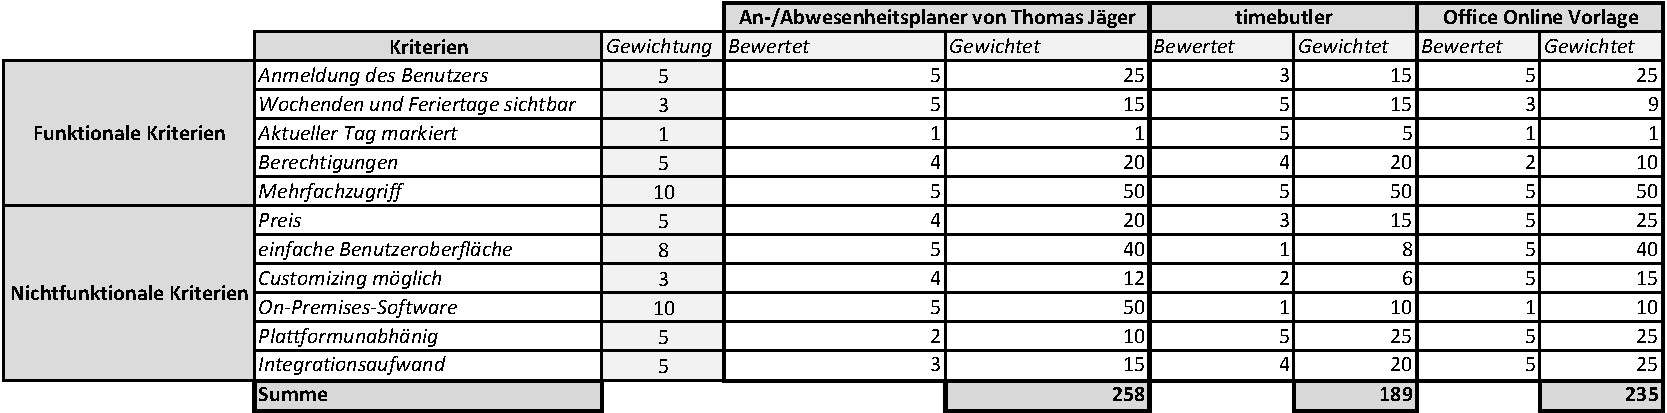
\includegraphics[width=0.9\textwidth,angle=0]{abb/Markterkundung.pdf}
    \caption[Beschreibung]{ Tabelle Markterkundung}
    \label{tab:Markterkundung}
\end{figure}

\subsubsection{An-/Abwesenheitsplaner von Thomas Jäger}
\label{sec:AnAbwesenheitsplaner}
Die erste betrachtete Software, der An-/Abwesenheitsplaner von Thomas Jäger, zeichnete sich durch die besonders intuitive Benutzeroberfläche aus. Bei der Betrachtung der anderen funktionalen Kriterien wurde festgestellt, dass die Software alle benötigten Anforderungen erfüllt und damit für den Einsatz geeignet ist. Negativ zu bewerten ist allerding, das die Software nur als Windows Programm zur Verfügung steht und damit nicht Plattformunabhängig eingesetzt werden kann. Zudem müsste ein solches Programm auf jedem Client PC im SMK installiert werden um die Software für alle Nutzbar zu machen. Damit ergibt sich ein hoher initialer Integrationsaufwand und auch späterer Wartungsaufwand den es zu berücksichtigen gilt. (vgl. \cite{AnAbwesenPlaner})


%Die Benutzerfreundlichkeit wurde jedoch als etwas komplex und steil eingestuft, was eine gewisse Einarbeitungszeit erforderte. Zudem war der Support nur eingeschränkt verfügbar und die Preisgestaltung vergleichsweise hoch. (vgl. \cite{AnAbwesenPlaner})
\subsubsection{timebutler}
\label{sec:timebutler}
Das zweite Programm namens timebutler überzeugte hingegen durch seine Plattformunabhängigkeit. Damit könnte es ohne großen Integrationsaufwand im SMK eingeführt und betrieben werden. Die Software bietet alle geforderten Funktionalitäten hat jedoch eine komplizierte Benutzeroberfläche und stellt viele Funktionen bereit die nicht benötigt werden. Das resultiert in höheren Anschaffungskosten als bei dem An-/Abwesenheitsplaner von Thomas Jäger. Besonders negativ ist zu bewerten, dass die Software zwar Plattformunabhängig ist, da sie auf Webtechnologien aufbaut, jedoch nicht als On-Premises-Software verfügbar ist. Damit müsste auf die Cloud des Anbieters zurückgegriffen werden was nicht gewünscht ist. (vgl. \cite{timebutler})

\subsubsection{Online Office Datei}
\label{sec:OnlineOffice}
Die dritte betrachtete Lösung ist die Verwendung einer Online Tabellenkalkulations Vorlage. Das würde es ermöglichen, die bereits vorhandenen Excel Tabellen für die Anwesenheitsplanung weiter zu verwenden. Durch das zurückgreifen auf Online Funktionalitäten die \zB von Microsoft mit Office356 oder mit Onlyoffice in Verbindung mit Nextcloud zur Verfügung stehen, kann man den gleichzeitigen Zugriff auf diese Listern erreichen. Damit würde man das Hauptproblem der einfachen Excel Dateien lösen. Doch auch hier müsste man im Falle des einsatzes von Office356 auf die Microsoft Cloud zurückgreifen. Desweiteren gibt es nur begrenzte Möglichkeit diese Excel Listen vor ungewollter Änderungen zu schützen und ein Berechtigungskonzept durchzusetzten.

\subsubsection{Auswertung der Marktrecherche}
\label{sec:AuswertungMarktrecherche}
Nach Betrachtung der drei Programme wurde festgestellt, dass keines der drei für eine Akquisition in frage kommt, da jedes seine individuellen Schwachstellen mit sich bringt. Der An-/Abwesenheitsplaner von Thomas Jäger wäre von allen die beste Option, da es eine benutzerfreundliche Oberfläche, eine solide Funktionalität und eine angemessene Preisgestaltung vereint. Die Plattformunabhängigkeit ist jedoch im SMK ein großer Faktor, da sich das neue Programm möglichst gut in die vorhandene Infrastruktur einfügen soll. Deswegen wurde sich gegen eine Akquisition von Standartsoftware entschieden. Um die geforderten Funktionalitäten abzubilden ohne dabei die Schwachstellen der Analysierten Programme inkauf nehmen zu müssen wurde ich für eine Eigenentwicklung der Software entschieden.

\subsection{Eigenentwicklung}
\label{sec:Eigenentwicklung}
Für die Umsetzung wurde Referat 12 mit der Entwicklung der Softwarelösung beauftragt. Die benötigten Hard- und Softwareressourcen vom SMK bereitgestellt und der zeitliche Rahmen für das Projekt wurde mit 32 Arbeitstagen angesetzt. Die genaue Aufschlüsselung des Projektablaufes siehe \ref{abb:Gantt}.

Für die Entwicklung der Software sethen dem Entwickler ein voll ausgestatteter Arbeitsplatz, sowie mehrere virtuelle Maschinen im Rechenzentrum zur Verfügung. Damit hat der Entwickler freie Hand bei der Umsetzung. Zu beachten ist jedoch, dass nach Möglichkeit auf die bestehende Infrastruktur zurückgegriffen bzw. berücksichtigt wird.


\subsection{Umsetzungsvarianten}
\label{sec:Umsetzungsvarianten}
Nach eingehender Analyse der Anforderungen und der Markterkundung wurden verschiedene Umsetzungsvarianten für das geplante Softwareprojekt des Anwesenheitsplaners untersucht. Dabei wurden insbesondere zwei Ansätze für die Entwicklung betrachtet: die monolithische Anwendung und eine Client-Server-Anwendung. Dabei handelt es sich um verschiedene Architekturen mit Vor- und Nachteilen. Architekturen sind in der Softwareentwicklung nicht unbedingt einheitlich Definiert weshalb in den folgenden Absätzen eine gemischte Betrachtung aus der System- und Software Architektur durchgeführt wird. Zusätzlich soll auch auf praktische Umsetzungsvarianten der einzelnen Architekturen eingegangen werden um ein praktisches Beispiel zu geben.

Es soll noch keine Betrachtung des Software Design Patterns angestellt werden, da dieses für den Auswahlprozess der Plattform noch keine Rolle spielt. Dementsprechen wird bei der bergachtung nur erwogen welchen Systemansatz man für die Umsetzung des Projektes wählen sollte.
%Es Softwararchitektur ist vielseitig ...Webbasiert ... Systemarchitektur... Disigneentscheidungen mvvm...

\subsubsection{monolithische Architektur}
\label{sec:monolithisch}
%TODO:was ist monolitisch
Die historisch klassische Form ist die monolithische Architektur. Beim dieser entsteht eine eigenständige Anwendung, die \zB direkt auf den Client PCs installiert wird. Bei diesem Ansatz ist die Software in der Lage, alle erforderlichen Komponenten und Dienste selbst bereitzustellen. Das ist vor allem dann geeignet, wenn die Anwendung auf einer spezifischen Plattform ausgeführt werden soll und keine Notwendigkeit für eine verteilte Architektur besteht. Da die monolithische Architektur sowohl das User-Interface als auch die Logik in einem Prozess beinhaltet, entfällt der zusätzliche Bedarf an einem dedizierten Server zum bearbeiten der Logik. Nachteil hierbei ist die eingeschränkte Flexibilität, da ein solches Programm an das System gebunden ist für das es Entwickelt wurde.

\subsubsection{Client-Server-Architektur}
\label{sec:ClientServer}
%TODO:Was ist Clien-Server
Die zweite betrachtete Option war die Client-Server-Architektur, die bei webbasierten Anwendungen mit einem Backend-Server und einer Datenbank zum Einsatz kommt. Bei dieser Architektur werden die Funktionen auf mehrere Schichten aufgeteilt. Der Backend-Server ist für die Verarbeitung der Anfragen und die Bereitstellung von Daten zuständig, während die Datenbank die persistente Speicherung der Daten ermöglicht. Der Benutzer interagiert mit der Software über das Frontend, das auf dem Client läuft. Um eine Verbindung zwischen Frontend und Backend herzustellen sendet der Client Anfragen an den Server und erwartet entsprechende Antworten mit Daten. Die Kommunikation zwischen Client und Server erfolgt dann über ein Netzwerkprotokoll wie HTTP. Ein Nachteil ist dabei die ständige Netzwerkabhängigkeit der Clients um den Dienst Nutzen zu können und eine erhöhtes maß an Komplexität in der Entwicklung gegenüber der monolithische Architektur.

Als weiterentwicklung der Client-Server-Architektur kommen auch noch die Service Orientierte Architektur (SOA) und die Micro Service Architektur in frage. Diese beiden Architekturansätze erlauben das Backend in kleinere einzeldienste zu zerlegen die dann unabhängig voneinander entwickelt, betrieben und skaliert werden können. Das ist ein großer Vorteil bei besonders großen Projekten in denen verschiedene Technologien und Programmiersprechen eingesetzt werden oder ein sehr hohes Maß an Lastverteilung gefordert ist. Für Projekte mit mittel bis kleinem Umfang ist eine solche Architektur jedoch nicht optimal, da das level an Komplexität extrem steigt und die Vorteile der Architekturen warscheinlicht nicht ausgeschöpft werden können.

\subsubsection{Vergleich}
\label{sec:Vergleich}
Beide der Architekturansätze könnten für den Anwesenheitsplaner eingesetzt werden. Der monolithische Ansatz würde in eine Anwendung für die Windows Clients im SMK münden. Die Software könnte dann als eine Windows Forms oder WPF (Windows Presentation Foundation) Anwendung erstellt werden, was den Vorteil hätte das die Logik und die GUI direkt miteinander verbunden wären und so ein direkter Zugriff auf Benutzereingaben während der Laufzeit möglich ist. Ein weiterer Vorteil ist, dass schon viele Kenntnisse bei der Csharp und Windows Forms Entwicklung vorhanden sind. (vgl. \cite{wpf}, \cite{modernApp})

Eine Client-Server-Architektur in Hinsicht auf eine Browserbasierte Bereitstellung bietet sich ebenfalls an. Die Vorteile eines Webbasierten Ansatzes sind ein sehr hohes Maß an Flexibilität bei den Zielplattformen der Clients und damit eine hohe Zukunftssicherheit. Im Kontext des Projektes des Anwesenheitsplaners bedeutet das, dass der Anwesenheitsplaner auf jedem Gerät im SMK aufgerufen werden kann. Das ist ein wichtiger Faktor, da viele Bedienstete mit moblien Geräten wie Smartphones und Tablets ausgestattet sind. Webbasierte Anwendungen müssen im gegensatz zu Desktop Entwicklungen wie Windows Programmen oder Smartphone Apps nicht installiert werden, das diese von einem zentralen Server bereitgestellt werden und nur von Browser angezeigt werden.

Negative Punkte bei einer Client-Server-Architektur gerade bei Betrachtung von Webtechnologien die erheblich steigende Komplexität. Durch die Trennung von Frontend und Backend muss eine Möglichkeit zur Kommunikation über Schnittstellen geschaffen werden. Das sorgt für eine eingeschränkte Interaktion des Nutzers mit der Logik was zu schlechterer Leistung von Webanwendungen im Vergleich zu Decktopanwendungen führen kann. Um diese Nachteile auszugleichen sollten moderne Frameworks für die Webentwicklung eingesetzt werden. Im Bereich der Webentwicklung ist der Kenntnisstand der Entwickler etwas geringer als bei Decktopanwendungen, was für die Umsetzung Verzögerungen bedeuten könnte. Es sollte also bei diesem Ansatz ein möglichst vertrautes Framework für die Entwicklung verwendet werden.

\subsubsection{Entscheidung}
\label{sec:Entscheidung}
Nach sorgfältiger Abwägung der Vor- und Nachteile beider Ansätze wurde beschlossen, auf eine Client-Server-Architektur mit einer Website als Frontend und einem Webserver als Backend zu setzen um so die Plattformunabhängigkeit von Webtechnologien nutzen zu können. Insgesamt bietet die gewählte Architektur die besten Voraussetzungen für die Umsetzung des Anwesenheitsplaners. Durch eine Webentwicklung wird eine flexible, plattformunabhängige Anwendung geschaffen, die sowohl auf Desktop PCs als auch auf mobilen Geräten und Virtuellen Citrix Maschinen genutzt werden kann ohne neue installationen vornehmen zu müssen.





\section{Entwurf}
\label{sec:Entwurf}
In der Entwurfsphase sollen aus den Anforderungen Modelle der zu entwickelten Software entstehen, die die konkreten Hardware- und Softwarebezogenen Anforderungen berücksichtigen. Diese Modelle gelten dann als unmittelbare Vorlage für die sich anschließende Implementationsphase. (vgl. \cite[S. 69]{dumke-2003})

UML-Diagramme sind unter anderem ein effektives Werkzeug, um den Programm- und Datenentwurf zu unterstützen und zu dokumentieren. Letztendlich soll mithilfe geeigneter Modelle ein Entwurf der zu Implementierenden Software erarbeitet werden. Dies umfasst die Festlegung des Softwaredesignes, der Datenstruktur und der grafische Oberfläche.

Bei der Erstellung des Entwurfes müssen die Datensicherheitsanforderungen beachtet werden. Dafür sollte im Fall dieses Projektes der Leitfaden zur Entwicklung sicherer Webanwendungen und der IT-Grundschutz-Baustein CON.8 Software-Entwicklung des BSI beachtet werden. Diese enthalten funktionale und nichtfunktionale Anforderungen die bei er Implementierung beachtet werden müssen. So wird in BSI CON.8 ein sicheres Systemdesigne gefordert. Dafür müssen \ua die folgenden Anforderungen beachtet werden:
\begin{itemize}
    \item  \gqq{Zur Benutzer-Authentisierung und Authentifizierung MÜSSEN vertrauenswürdige Mechanismen verwendet werden, die den Sicherheitsanforderungen an die Anwendung entsprechen} (\cite[S.5]{BSICON8})
    \item  \gqq{Sicherheitsrelevante Ereignisse MÜSSEN in der Art protokolliert werden, dass sie im Nachgang ausgewertet werden können} (\cite[S.5]{BSICON8})
    \item  \gqq{Schützenswerte Daten MÜSSEN entsprechend der Vorgaben des Kryptokonzepts verschlüsselt übertragen und gespeichert werden} (\cite[S.5]{BSICON8})
\end{itemize}

Im Leitfaden zur Entwicklung sicherer Webanwendungen werden spezifisch für Webserver geeignete Sicherheitsanforderungen definiert. Beispielsweise wird eine Zugriffskontrolle, bei der Objektzugriffe auf vorhandene Berechtigungen geprüft werden, gefordert. Ebenfalls soll generell das Least Privilege Konzept verfolgst werden, bei dem jede Komponente oder Benutzer nur die nur die notwendigen Berechtigungen besitzt um eine Aktion auszuführen. (vgl. \cite{BSIWeb})

%TODO:QUELLE https://www.bsi.bund.de/SharedDocs/Downloads/DE/BSI/Publikationen/Studien/Webanwendungen/Webanw_Auftragnehmer.pdf?__blob=publicationFile&v=1

\subsection{Logikentwurf}
\label{sec:Logikentwurf}
%TODO:MVVM
Der Logikentwurf soll basierend auf dem Use-Case-Diagramm, siehe Abbildung \ref*{fig:Use-Case-Diagramm} entstehen. Dabei sollen aus den Anwendungsfällen die benötigten Funktionen des Programms erarbeitet werden. Für einen ersten Überblick des gesamten Prozesses wurde ein Ablaufdiagramm erstellt was die Prozessschritte mit den benötigten Datenquellen zeigt, siehe Abbildung \ref*{abb:Flow}.

Die Anwendung soll als erstes den Nutzer authentifiezieren um die Berechtigungen feststellen zu können. Wenn der Nutzer berechtigt ist wird seine Referatszugehörigkeit mittels des AD ermittelt. Nach dem Login Prozess werdem dem Nutzer im Frontend die Anweseheitsdaten seiner Kollegen das aktuellen Monats angezeit. Dort kann er seine eigenen Anwesenheiten ändern oder in den Monatsansichten vor und zurück springen. Jede änderung eines eigenen oder im Falle eines Admins, eines Datensatzes im generellen wird direkt an die Datenbank übermittelt und dort gespeichert.

Um die einzelnen Prozessschritte als Funktionen näher zu beschreiben wurden Programmablaufpläne (PAP) erstellt. Beispielhaft ist im Anhang \ref{abb:PAP} der PAP für die Funktion des Änderns von Anwesenheiten.

\begin{figure}[htb]
    \centering
    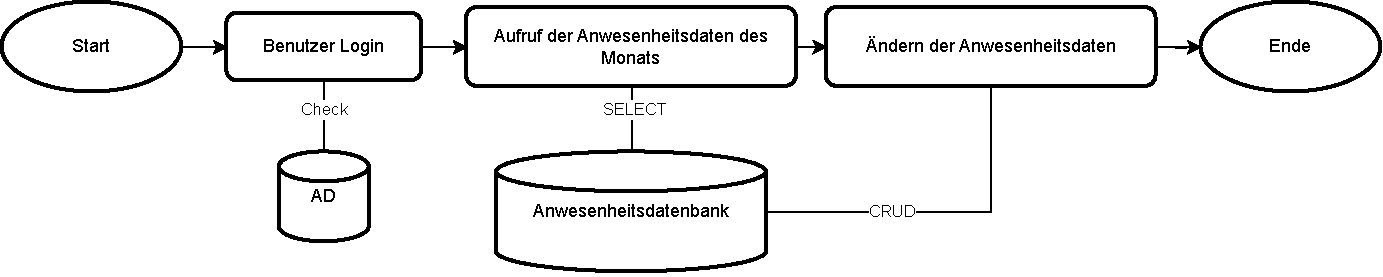
\includegraphics[width=0.9\textwidth,angle=0]{abb/Flow-Diagramm.drawio.pdf}
    \caption[Beschreibung]{Ablaufdiagramm}
    \label{abb:Flow}
\end{figure}

\subsection{Softwaredesigne}
\label{sec:Softwaredesigne}
Für die Umsetzung des Logikentwurfs mit dem Blazor Framework soll eines der beiden in Absatz \ref{sec:Framework} \nameref{sec:Framework} aufgezeigten Muster implementiert werden. Es konnten sowohl mit MVC als auch mit MVVM bereits Erfahrungen gesammelt werden und deshalb wurde die Entscheidung für ein Muster hauptsächlich aus individuellen Gründen getroffen. Das MVVM Muster ist übersichtlicher und wurde in anderen Projekten bereits erfolgreich umgesetzt. Dasswegen fiel die Wahl auf den einsatz des MVVM Musters.

Damit ergibt sich die Strukturierung des Softwarekomponenten die für das Projekt benötigt werden. Es werden Model Klassen benötigt die, die Anwesenheitsdaten repräsentieren und in der Datenbank persistent gespeichert werden. Das ViewModel ist ebenfalls eine Klasse die, die gesamte Funktionalität für eine View beinhaltet. Damit wird pro View ein ViewModel erstellt. Die View ist nur für die Darstellung zuständig und ist ein HTML Tamplate in das dynamisch Werte aus dem ViewModel gerendert werden.
%TODO:Quelle:https://learn.microsoft.com/de-de/dotnet/architecture/maui/mvvm

Für eine bessere übersicht und ggf. wiederverwendbarkeit von Code sollen für die Datenbankkommunikation und die AD integration eigene bzw. vorhandene Bibliotheken verwendet werden die dann im ViewModel verwendet werden. Für die AD Abfragen soll eine Klassenbibliothek AD Manager erstellt werden und für die Datenbankkommunikation eine DataAccessLibrary. Diese Datenbankkommunikationsbiblithek soll dann die Grundlage für die Datenbankoperationen wie Laden oder Speichern von Daten in der Geschäftslogik sein. In der Geschäftslogik werden diese Methoden zu Laden oder Speichern mit einem SQL Befehl und Objekten an diese Bibliothek übergeben und diese übernimmt dann die Datenbankkommunikation. Das auslagern dieser Basisfunktionalität hat den Vorteil, dass es in anderen Projekten wieder eingesetzt werden kann.

\subsection{Systementwurf}
\label{sec:Systementwurf}




\subsection{Datenentwurf}
\label{sec:Datenentwurf}
Um die Daten aus dem Anwesenheitsplaner in eine Datenbank zu speichern muss dafür eine neue, mit passendem Schema, Angelegt werden. UML-Diagramme wie das ERM können dabei verwendet werden, um die Tabellenstruktur, die Beziehungen zwischen den Tabellen und die Attribute zu modellieren. Dies ermöglicht eine klare Darstellung der Datenbankstruktur und hilft dabei, die Datenintegrität und -konsistenz schon in der Planung sicherzustellen. Durch diese Art an Dokumentation ist es auch möglich bei der Entwicklung des Programms passende Klassen für die Verarbeitung der Daten aus der Datenbank herzuleiten.

Die zu speicherten Daten ergeben sich aus der in der Analysephase erhoben Tabelle im Abbildung \ref{abb:Ausgangstabelle}. Um die Daten möglichst simpel aus der Datenbank auslesen und zurückschreiben zu können, sollte versucht werden die Datenstruktur so anzulegen das die Daten in einem in der Programmlogik gut verarbeitbares Schema gespeichert werden. Um möglichst einfache Abfragen zu ermöglichen wurde keine Normalisierung der Tabellenstruktur durchgeführt um Zeit zu sparen. Um später Fehler zu vermeiden könnte das Schema für eine weiterentwicklung angepasst werden. Im aktuellen Fall wurde sich gegen eine Normalisierung entschieden, da die Prüfung der eingaben auf der Frontendseite geschehen soll.

Für das Anlegen der Datenstrukturen im Programmcode und in der Datenbank wurde ein Entity-Relationship-Modell (ERM), siehe \ref{abb:ERM} erstellt. Hier soll es zwei Tabellen geben, die Tabelle Person wird zum Teil aus dem AD befüllt und hält zum Teil Informationen die für Funktionen des Anwesenheitsplaners benötigt werden. Die Tabelle Anwesenheit beinhaltet alle Anwesenheitseinträge der Nutzer. Dem Nutzer wird eine ein Anwesenheitseintrag über die Verbindung mit seinem Sicherheitsbezeichner (SID) im AD zugeordnet. Die SID wird benötigt da sich der Name des Nutzers ändern kann und damit nicht als Primärschlüssel eignet. Die SID wird vom AD beim erstellen des Kontos angelegt und ändert sich nie. (vgl. \cite{sid})

\begin{figure}[htbp]
    \centering
    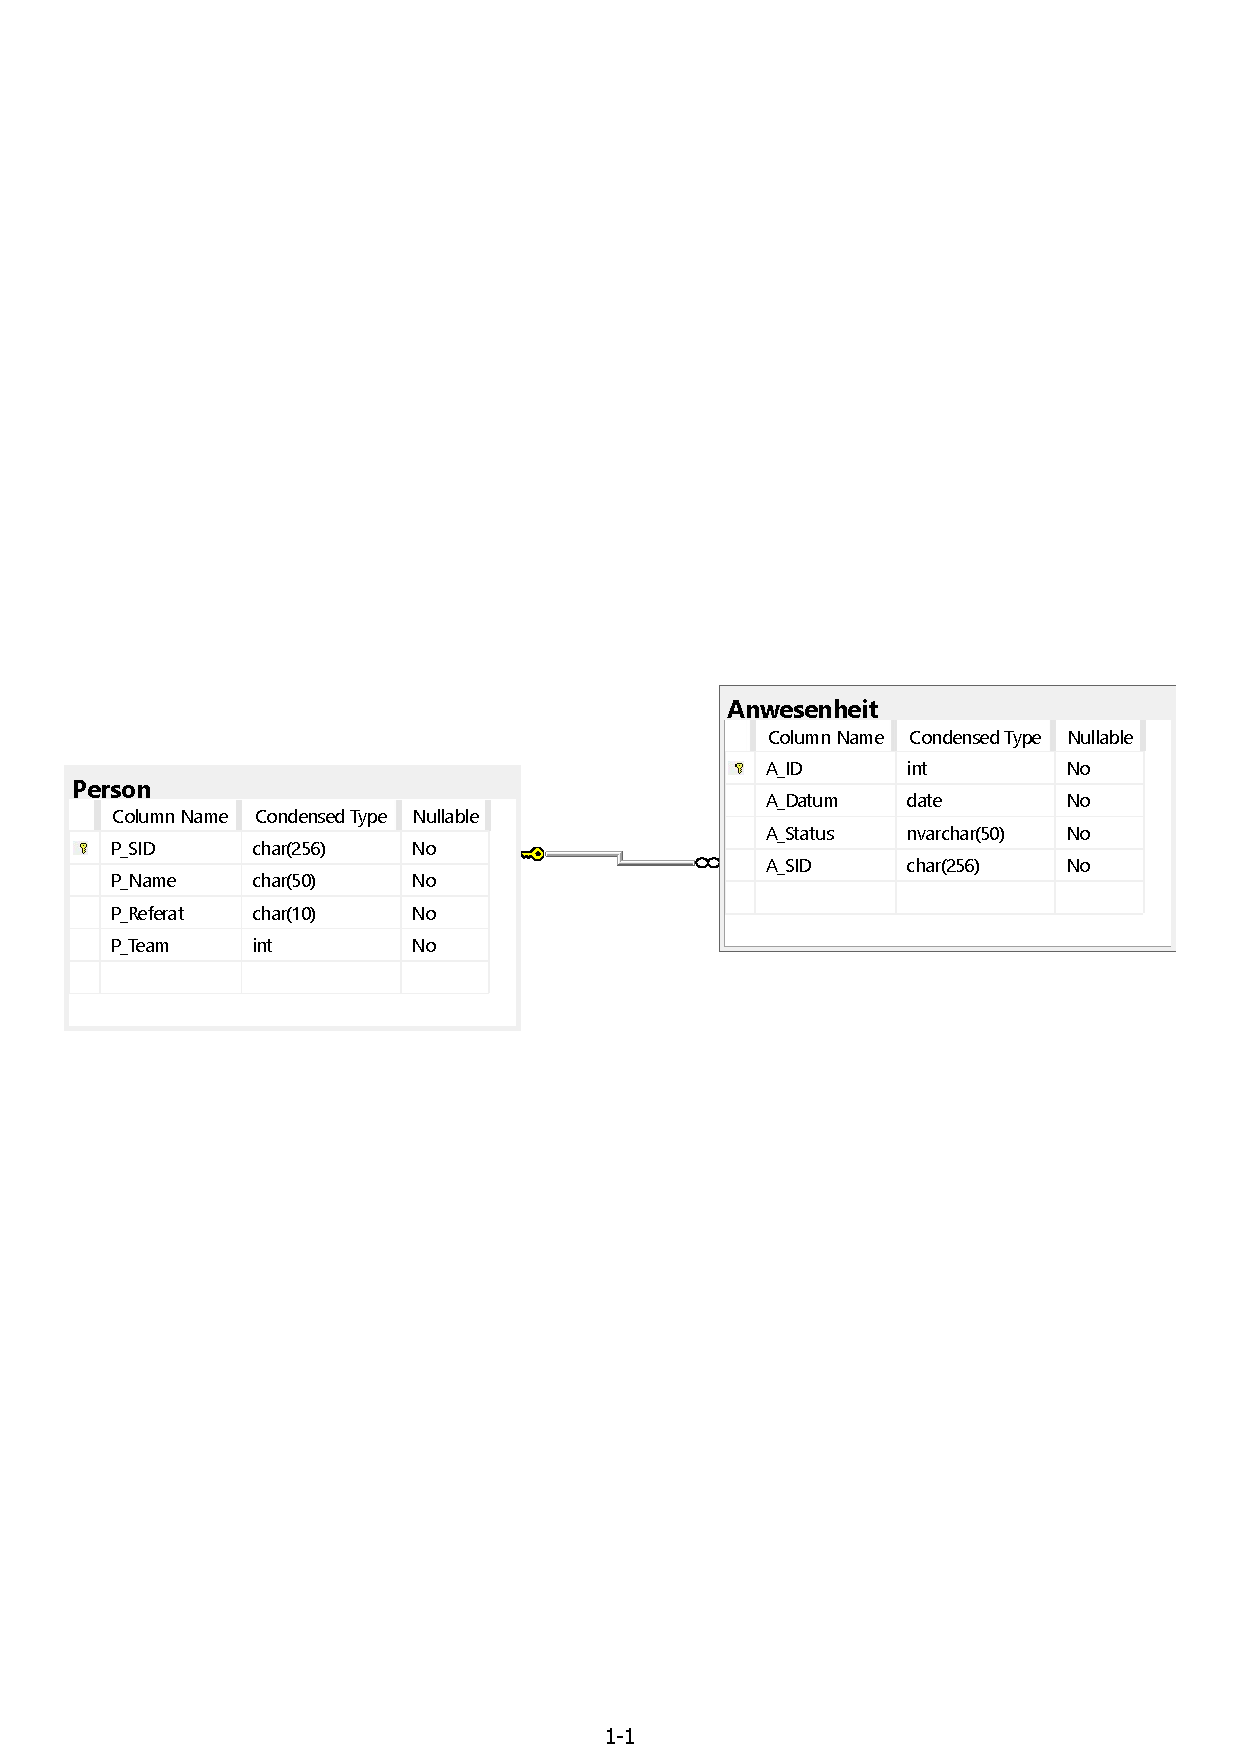
\includegraphics[width=0.9\textwidth,angle=0]{abb/ERM.pdf}
    \caption[Beschreibung]{ERM}
    \label{abb:ERM}
\end{figure}
%TODO:ERM erklären mit Quelle?


\section{Implementierung}
\label{sec:Implementierung}
In der Implementierungsphase wird die Software gemäß der Anforderungen und Spezifikationen aus \nameref{sec:Analysephase} und \nameref{sec:Entwurf} umgesetzt. Der Entwicklungsprozess ist in mehrere Phasen unterteilt, darunter die Programmierung, das Testen und letztlich die Migration ins Livesystem.

Auf Grundlage der in der im \nameref{sec:Entwurf} angefertigten Modelle wurden daraus konkrete Datenstrukturen und Algorithmen umgesetzt. Während der Implementierungsphase wurde besonderes Augenmerk auf die Modularität und Wiederverwendbarkeit des Codes gelegt, um die spätere Erweiterbarkeit der Software zu erleichtern.

\subsection{Kernmodule des Anwesenheitsplaners}
\label{sec:Kernmodule}
Die Entwicklung umfasste mehrerer Kernmodule, die jeweils spezifische Aufgaben und Funktionen der Software erfüllten. Diese werden in den folgenden Sektionen näher vorgestellt. Dabei wird zuerst auf das zu lösende Problem kurz eingegangen und dann die Lösung für den Anwesenheitsplaner erläutert. Dafür wird \ggfs auch Bezug auf Codesegmente genommen, die sich im Anhang befinden. Eine Übersicht über alle Klassen ist in Abbildung \ref{abb:Klassendiagramm} im Anhang ersichtlich.

\subsubsection{AD Manager}
\label{sec:ADManager}
Die Kernfunktionalität des Anwesenheitsplaners ist es, einem Nutzer nach Anmeldung an der Weboberfläche die Anwesenheiten seiner Referatsmitglieder anzuzeigen. Dafür muss dem Programm allerdings bekannt sein, in welchem Referat sich der Benutzer befindet, damit für Ihn passende Einträge aus der Datenbank geladen werden können. Diese Informationen stellt die Klasse AD Manager bereit.

Bei der Anmeldung an der Weboberfläche wird der Benutzer durch seine bereits erfolgte Windows Anmeldung durch den IIS als Benutzer erkannt. Dadurch kann über das .NET Framework auf den angemeldeten Benutzer als UserPrincipal Klasse zugegriffen werden. Mit diesem Objekt kann man nun über eine AD Abfrage vom aktuellen Benutzer den AD Wert für department auslesen. Somit kann aus dem AD für den Nutzer das richtige Referat ermittelt werden. Diese Funktionalität wird über GetUserInfo() umgesetzt. Diese Methode gibt noch eine weitere wichtige Information, die SID des Benutzers zurück. Die SID dient zur eineindeutigen Identifizierung des Nutzers und wird in der Datenbank als Primärschlüssel für die Nutzer verwendet. Die gefundenen Informationen werden dann als Dictionary an die Geschäftslogik übergeben. Hier könnten falls nötig sehr einfach weitere Informationen für die Anwendung angefügt werden.

Die zweite Funktionalität ist die GetPersonsInDepartment(string department) Methode. Diese wird genutzt, um für den aktuellen Benutzer die zugehörigen Einträge für alle Rederatsmitglieder zu erhalten. Das Referat des angemeldeten Benutzers wird in die Methode übergeben und diese durchsucht dann mit einem PrincipalSearcher das AD in der SMK OU nach den passenden AD Konten, die auch dem Referat angehören und gibt diese zurück.

Der AD Manager wird dann in der Datenlogik aufgerufen und die Rückgabewerte werden für die Interaktion mit der Datenbank benötigt. Ohne eine Verbindung zum AD kann der Anwesenheitsplaner also nicht funktionieren.

\subsubsection{Daten und Datenlogik}
\label{sec:Daten}
Für die persistente und zentrale Speicherung der Anwesenheitsdaten wurde ein relationale Datenbank ausgewählt. Um die Daten aus der Datenbank zu lesen und neue oder aktualisierte Daten zu schreiben, wird eine Schnittstelle zur Datenbank benötigt. Dort wurde sich gegen den Einsatz des weit verbreiteten Entity Frameworks entschieden, da dieses Framework eine ausgewachsener Microsoft Object Relational Mapper (ORM) ist. Damit ist es die wichtigste .NET-Datenzugriffs-API. Jedoch kann der Einsatz einer ORM sehr komplex werden und im Fehlerfall für ungeübte Entwickler zu großen Verzögerungen bei der Fehlerbehebung führen. Deswegen wurde die Mikro-ORM Dapper verwendet.

Dapper ist eine von den Stack Overflow Entwicklern geschriebene Open-Source ORM, die besonderen Fokus auf Optimierung des Datenzugriffs legt. Bei der Nutzung von Dapper schreibt der Entwickler die SQL Befehle selbst und Dapper bietet Transformationsfunktionen wie \zB das Einbetten von Objekten in den SQL Befehl oder das Umwandeln von Datensätzen aus der Datenbank in Listen an. Das macht den Datenbankzugriff sehr intuitiv und Fehler können schnell gefunden werden, da die SQL Befehle im Code sichtbar sind. Dapper implementiert auch eingebaute Funktionen gegen SQL Injections und erhöht somit die Datensicherheit. Durch die Kombination aus einfachen SQL Befehlen und der sehr guten Transformationsmechanik von Dapper können die Daten sehr einfach aus der Datenbank und auch in die Datenbank geschrieben werden. (vgl. \cite{Dapper})

Alle Interaktionen mit der Datenbank wurden über die Einbindung von Dapper gelöst. Dafür wurden die Klassen SQLDataAccess und SQLDataAccessAsync erstellt. Diese beinhalten ausschließlich Methoden zum Speichern und Laden von Daten unter Verwendung von Type T. Damit konnten Templates für die Methoden zum Synchronen und Asynchronen Datenzugriff mit der Verwendung von Dapper erstellt werden, die dann der Geschäftslogik zur Verfügung stehen. Ein Beispiel für ein solches Tamplate ist im nachfolgendem Codebeispiel \ref{lst:LoadDataAsync} zu sehen.
\\

\begin{lstlisting}[frame=single,caption={Die Methode {\normalfont \ttfamily  LoadDataAsync} aus der SQLDataAccessAsync Klasse}, label={lst:LoadDataAsync}]
public async Task<List<T>> LoadDataAsync<T, U>(string sql, U parameters)
{
    string connectionString = _config.GetConnectionString(ConnectionStringName);

    using (IDbConnection connection = new SqlConnection(connectionString))
    {
        var data = await connection.QueryAsync<T>(sql, parameters);

        return data.ToList();
    }
}
\end{lstlisting}

Die die gesamte Geschäftslogik für das Speichern und Schreiben der Daten wurde in Klasse UserData ausgelagert. Die Methoden der Klasse UserData bilden eine Operation, wie \zB das Laden der Anwesenheitsdaten eines Nutzers, ab. Dabei sind diese Methoden für genau diesen Anwendungszweck ausgelegt und werden dann bei der Bearbeitung der Events aus dem Frontend ausgelöst.

Am schwierigsten gestaltete sich dabei die Implementierung, das Lesens der Anwesenheitsdatensätze aus der Datenbank. Gespeichert sind diese, wie in Abbildung \ref{abb:ERM} zu sehen, mit SID, Datum und Anwesenheitsstatus. Im Model für die View wird das Tupel aus Datum und Anwesenheitsstatus als Dictionary dem Objekt deines Nutzers zugeordnet. Um die Leistung zu verbessern, wurde sich dazu entschlossen, die Fähigkeit von Dapper, Klassen Attribute auf Datenbank Attribute zu Mappen zu nutzen, indem man durch das geschickte Nutzen der Aliase in SQL mittels Key und Value Zuordnung direkt ein Dictionary befüllt, was dann unter Angabe der SID des zugehörigen User-Objektes dem passenden Objekt als Rückgabewert zugeordnet werden kann.
\\
\begin{lstlisting}[frame=single,caption={Die Methode {\normalfont \ttfamily  GetUserDateStat} aus der UserData Klasse}, label={lst:GetUserDateStat}]
public Task<Dictionary<DateTime, string>> GetUserDateStat(string sid, int month)
{
    string sql = @"
    SELECT DISTINCT A_Datum AS[Key], A_Status AS[Value]
    FROM dbo.Anwesenheit WHERE A_SID = @SID AND MONTH(A_Datum) = @MONTH
    ";

    return _dbasync.LoadDataDictAsync<Dictionary<DateTime, string>, dynamic>(
        sql, new {
            SID = sid, MONTH = month
        });
}
\end{lstlisting}

\subsubsection{View}
\label{sec:View}
Für das Frontend sollte eine einfache Benutzeroberfläche entstehen, welche der Excelliste stark ähnelt und nur die benötigten Funktionalitäten bereitstellt. Es muss also eine Tabelle in HTML gerendert werden, die als Tabellenkopf die Referatsmitglieder in seperaten Spalten beinhaltet sowie zudem die Daten der Tage im Monat. Bei einem Klick auf ein Datumsfeld, was in der eigenen Spalte liegt, soll dann der zuvor Ausgewählte Anwesenheitsstatus eingetragen werden, der dann wiederum an die Geschäftslogik und damit auch in die Datenbank übertragen wird.

Für die Erstellung der Benutzeroberfläche wurden die vom Framework vorgegebenen ASP.NET Core Razor Pages verwendet. Dabei handelt es sich um auf dem Server gerenderten Benutzeroberfläche. Durch den Einsatz des Blazor Server Frameworks in Verbindung mit Razor Pages kann nun View-spezifische Logik für die Seite implementiert werden. Des Weiteren verwendet das Framework die Razor Syntax, welche es ermöglicht Csharp Code direkt in HTML einzubetten. Somit lassen sich leicht interaktive Benutzeroberflächen erstellen, die auf Csharp Code basieren. (vgl. \cite{Razor}, \cite{RazorSyntax})

Die Geschäftslogik befindet sich angegliedert an die View. Dort sind konkrete Event Handler für die Benutzeroberfläche hinterlegt, die dann \zB mit der Datenbank über die UserData Klasse kommunizieren oder die Berechtigungen des Benutzers prüfen. Dabei sind die in das HTML eingebetteten Objekte direkt in der Geschäftslogik integriert. Das ermöglicht die dynamische Generierung der anzuzeigenden Tabelle, indem eine Schleife für jeden in der Liste an Referatsmitgliedern eine eigene Tabellenspalte erzeugt. Für den Nutzer wurde die Klasse UserModel erstellt. Beim initialen Aufruf wird für jedes Referatsmitglied ein Objekt dieser Klasse erzeugt und aus der Datenbank befüllt. Bei Änderungen eines Anwesenheitseintrages auf der Benutzeroberfläche wird die Änderung direkt in das Model des entsprechenden Referatsmitglieds übernommen, da das Objekt direkt in HTML eingebunden ist. Durch das Einbetten von UserModel Objekten in die dynamisch generierten Tabellenspalten können vollautomatisch sämtliche Variationen an Anzahl und Zusammenstellung des Referates abgebildet werden. %TODO: Codebeispiel im Anhang


\subsection{Tests und Qualitätssicherung}
\label{sec:Tests}
Die Durchführung von Tests während der Entwicklung und zum Abschluss ist besonders wichtig, um die Qualität und Zuverlässigkeit der Anwendung sicherzustellen. Dabei sollten alle wesentlichen Komponenten, nämlich das Frontend, die Datenbank und Datenlogik und die Geschäftslogik sorgfältig getestet werden. Während der Entwicklung wurden immer wieder Komponententests durchgeführt, um die partielle Funktionalität sicherzustellen. Das war besonders notwendig da alle Komponenten aufeinander aufbauen.

Nach der Implementation aller benötigten Funktionalitäten wurde ein Prototyp des Systems für erweiterte Tests verschiedenen Zielgruppen zur Verfügung gestellt. Um ein umfassendes Bild über die Funktionsfähigkeit der Software und die Aktzeptern bei den Nutzern zu bekommen, wurde der Prototyp sowohl dem Referat 12 als auch ausgewählten Mitarbeitern aus anderen Referaten vorgestellt. Durch Referat 12 wurde der Prototyp und das dazugehörige System mit Datenbank und Webserver auf System und Software Schwachstellen untersucht. Dabei wurde bei der Datenbank das Speichern- als auch das Abfragen von Daten getestet. Auch die Geschäftslogikkomponenten wurden auf ihre Funktionalität, die Verarbeitung von Eingabedaten und die korrekte Rückgabe von Ergebnissen hin überprüft.

Bei den Tests mit Mitarbeitern aus anderen Referaten wurde vor allem das Frontend getestet. Dabei lag der Fokus darauf, die Benutzeroberfläche auf verschiedenen Endgeräten und Browsern zu prüfen, sicherzustellen, dass alle Interaktionen reibungslos funktionieren und die Benutzerfreundlichkeit gewährleistet ist. Dabei wurden konkret die in Abbildung \ref{fig:Use-Case-Diagramm} definierten Anwendungsfälle geprüft.

Die Auswertung der Testphase ergab, dass die Anforderungen an das Anwesenheitsplaner-System noch nicht vollständig erfüllt sind. Insbesondere wurden drei Bereiche identifiziert, die Verbesserungen erfordern. Datenschutz und Datensicherheit müssen für eine im SMK eingesetzten Dienst weiter ausgebaut werden. Es müssen zusätzliche Schutzmaßnahmen implementiert werden, um sensible Informationen vor unbefugtem Zugriff zu schützen. Zweitens wäre ein Code Refactoring hilfreich, um die Codebasis zu optimieren und mögliche technische Schulden zu reduzieren, die aufgrund des engen zeitlichem Rahmens entstanden sind. Des Weiteren sollte die Fehlerbehandlung intensiviert werden, indem viele Szenarien durch entsprechende Fehlermeldungen und Serverseitige Validierung geprüft werden, um den Benutzern klare Rückmeldungen zu geben. Durch die gezielten Verbesserungen dieser Punkte soll die Webanwendung im Anschluss in einer zweiten Entwicklungsphase fertiggestellt und migriert werden.

\section{Fazit}
\label{sec:Fazit}
Im Fazit sollen die technische Implementierung der Software wie auch die Erfüllung der ursprünglichen Zielsetzung in Bezug zu den definierten Anforderungen analysiert und bewertet werden. Dabei werden die Projektphasen, die eingesetzten Technologien, die Qualität der Codebasis sowie die erreichten Funktionalitäten betrachtet. Des Weiteren werden etwaige Herausforderungen und Hindernisse während der Entwicklungsphase beleuchtet und mögliche Gründe für Abweichungen von der ursprünglichen Planung untersucht. Abschließend werden Empfehlungen zur Optimierung und Weiterentwicklung der Software formuliert.

\subsection{Zusammenfassung des Projektes}
\label{sec:Zusammenfassung}
Diese Arbeit widmete sich der Entwicklung eines neuen Anwesenheitsplaners für das SMK mit dem Ziel, die Probleme der bestehenden Lösung mit Excel zu beheben. Bei der Umsetzung wurde sich an den klassischen Phasen eines Softwareentwicklungsprojektes orientiert. Zuerst wurden die Probleme der bestehenden Lösung untersucht. Darauf folgend wurden mithilfe einer Anforderungsanalyse die funktionalen und nichtfunktionalen Soll-Kriterien erhoben. Nach der Analyse wurde eine ausführliche Variantendiskussion durchgeführt die sowohl die Akquisition von Standartsoftware als auch eine Eigenentwicklung in Betracht zog.

Es wurde sich für eine Eigenentwicklung entschieden, da keines der verglichenen Softwareprodukte passend war. Für die Eigenentwicklung wurden dann verschiedene Umsetzungsvarianten wie WebApps und Desktopanwendungen in Betracht gezogen. Am Ende wurde sich für die Entwicklung einer WebApp mit einer Monolith-Systemarchitektur entschieden. Als Framework für die Entwicklung wird Blazor Server eingesetzt.

Nach der Entscheidung für eine Umsetzungsvariante konnte auf Grundlage der Analyse dann der Software- und Systementwurf erstellt werden. Für den Entwurf der Geschäftslogik wurden Ablaufpläne und Klassendiagramme erstellt. Das System soll am Ende aus einem Webserver, der die WebApp hostet und einer Datenbank bestehen. Die Datenbank ist nur mit dem IIS Webserver verbunden und die Clients greifen ausschließlich auf den Webserver zu. Für die Erstellung der Datenbank wurde ein ERM angelegt auf Grundlage der Referenztabelle, siehe Tabelle \ref{abb:Ausgangstabelles}.

In der letzten Phase wurden der Entwurf implementiert. Dazu wurde die Datenstruktur in der Datenbank angelegt und die WebApp in Visual Studio entwickelt. Es konnten erfolgreich alle funktionalen Anforderungen implementiert werden, jedoch musste dafür bei der Datenlogik und der Implementierung des MVVM Modells technische Schuld aufgebaut werden. Am Ende konnte der entwickelte Prototyp von mehreren Mitarbeitern getestet werden. Dabei wurde sichtbar, dass der Abbau der technischen Schuld vor der Migration ins Live System notwendig ist, Datenschutz- und Datensicherheit gewährleistet werden müssen. Dementsprechend wird es eine zweite Entwicklungsphase geben müssen, in der die Fehler behoben werden sollen.

\subsection{Vorstellung des Prototypen}
\label{sec:Prototyp}
Als Ergebnis des Projektes konnte ein funktionsfähiger Prototyp entwickelt werden. Dieser ermöglicht es den Benutzern mit Single Sign-on auf die Weboberfläche des Anwesenheitsplaners zuzugreifen und dadurch die Anwesenheitsdaten zu verwalten. Die Benutzeroberfläche konnte sehr intuitiv gestaltet werden, was im Testverfahren mit den Mitarbeitern als sehr positiv aufgefasst wurde. Die gesamte Benutzeroberfläche des Prototypen ist in Abbildung \ref{abb:Prototyp} im Anhang einsehbar.

\begin{figure}[htb]
    \centering
    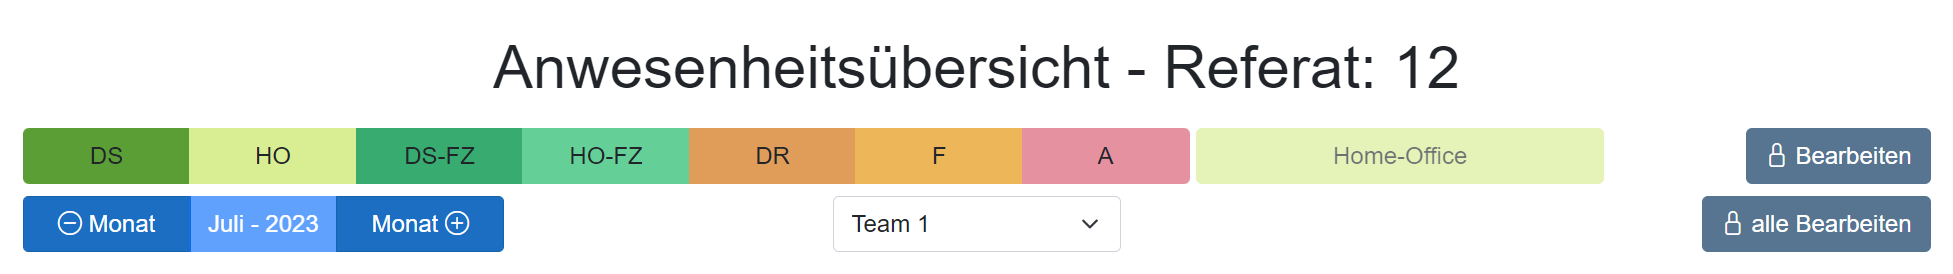
\includegraphics[width=1\textwidth,angle=0]{abb/Buttons_GUI.png}
    \caption[Beschreibung]{Schaltflächen}
    \label{abb:Buttons_GUI}
\end{figure}

Die Interaktion findet hauptsächlich über die Schaltflächen der Tabelle statt. Dort wird der gewünschte Anwesenheitsstatus ausgewählt, welcher anschließend durch das Klicken auf die Tabellenzelle für diesen Tag gesetzt wird. Die Schaltflächenübersicht ist in Abbildung \ref{abb:Buttons_GUI} zu sehen. Über die Schaltflächen \textit{Bearbeiten} und \textit{alle Bearbeiten} kann zwischen den Lese- \bzw Schreibmodus gewechselt werden. Dabei ist die Schaltfläche \textit{alle Bearbeiten} nur für Konten in der AD Gruppe AWPadmin mit einer Funktion hinterlegt.

Die Monatsansichten, links in blau, zeigen in der Mitte den aktuellen Monat und lassen sich mit den Schaltfläche links und rechts der Mitte um je einen Monat verschieben. Als letzte Schaltfläche kann der aktuell angemeldete Benutzer eine Teamzugehörigkeit auswählen, wodurch sich die Sortierung in der angezeigten Tabelle ändert. Damit können referatsinterne Substrukturen in dem Anwesenheitsplaner abgebildet werden.

Weitere Funktionen sind in Abbildung \ref{abb:Prototyp} im Anhang zu sehen. So sind \zB Feiertage und Wochenenden mit Gelb markiert und können keinen Anwesenheitsstatus bekommen. Der aktuelle Tag ist rot markiert wie im Falle der Abbildung der 18.07.2023.

\subsection{Soll-Ist-Vergleich}
\label{sec:Soll-Ist-Vergleich}
Der Soll-Ist-Vergleich zeigt, dass nahezu alle geplanten Funktionalitäten problemlos umgesetzt wurden. Die in der Use-Case-Analyse definierten funktionalen Anforderungen an das System wurden zufriedenstellend erfüllt. Das ist auf eine gute Analysephase zurückzuführen, da die Referenztabelle eine gute Vorlage für die zu entwickelnde Software bot. Allerdings haben die umfangreichen Tests auch einige Schwachstellen aufgezeigt. Insbesondere die Systemsicherheit und der Datenschutz müssen noch weiter ausgebaut werden, um den Prototypen auf den Einsatz in der produktiven Umgebungen vorzubereiten. Insbesondere ein Datenschutzkonzept, welches Aufbewahrungsfristen und den Umgang auf die Anwesenheitsdaten regelt, muss von der Datenschutzbeauftrageten im SMK abgesegnet werden. Auch müssen im Bereich der Datensicherheit noch Nachbesserungen erfolgen. Ein Kritikpunk stellt \zB das fehlende Logging in der WebApp dar. Zwar werden  standardmäßig vom Webserver und von der Datenbank Logs erzeugt, doch wird ein spezifisches Logging der Geschäftslogik gefordert. Ein weiter Punkt ist das alle Eingaben sowohl im Frontend als auch im Backend validiert werden, um Fehler zu minimieren und mögliche Angriffsvektoren zu schließen.

Abschließend ist zu sagen, dass der funktionale Soll-Zustand erreicht werden konnte, aber nur durch Abstriche in Codequalität und Sicherheitsfeatures, was auf den knapp bemessenen Zeitrahmen sowie fehlende Kenntnisse zurückzuführen ist.

\subsection{Bewertung der Umsetzung des Projektes}
\label{sec:Bewertung} %werden die Projektphasen,eingesetzten Technologien, die Qualität der Codebasis,Herausforderungen und Hindernisse während der Entwicklungsphase, Abweichungen von der ursprünglichen Planung
Die Umsetzung des Projektes verlief insgesamt erfolgreich, da durch eine solide Planung ein klarer Ablauf des Projektes definierte wurde. Dabei gab es in der Planung und Analyse keine nennenswerten Schwierigkeiten. Das änderte sich bei der Phase der Variantendiskussion, da keinerlei Vorwissen zu den Themen System- und Softwarearchitekturen vorhanden waren. Dies erschwerte den Prozess der Auswahl einer Umsetzungsvariante erheblich, da in der Folge das Wissen erst aufgebaut werden musste.

Die Auswahl der Technologien für die Umsetzung erwies sich im Nachhinein als sehr gelungen, sodass mit nur geringem Aufwand die benötigten Funktionalitäten realisiert werden konnten. Das gründete sich vor allem Dingen in der Wahl des Csharp basierten Blazor Server Frameworks. Dadurch konnte das vorhandene Csharp Vorwissen verwendet werden und ohne die Nutzung von Javascript eine funktionsfähige Weboberfläche erstellt werden. Nachteilig am Einsatz des Frameworks war die geplante Anwendung des MVVM Musters für die Benutzerinteraktionen. Durch den Aufbau einer Razor Page muss das MVVM Muster anders als bei vorher verwendeten Frameworks implementiert werden. Das führte dazu, dass das Muster nicht sauber implementiert werden konnte. Es resultierte eine zu niedrige Qualität der Codebasis, was schließlich in der zweiten Entwicklungsphase angegangen werden sollte.

Die größten Schwierigkeiten lagen in der Umsetzung der Datenschutz- und Datensicherheitsrichtlinien. Hier gab es während der Analyse-, Entwurf- und Implementierungs-Phase immer wieder Rücksprachen mit den verantwortlichen im SMK. Doch angemessene Maßnahmen für die geforderten Standards des BSI zu finden und diese Umzusetzen gestalten, stellte sich als viel zeitintensiver heraus, als erwartet. Deswegen musste von dem Plan ein für den Einsatz im Live System geeignete Software zu entwickeln Abstand genommen werden. Stattdessen wurde die Software als Prototyp zur Demonstration sowie für Tests verwendet, welche in einer zweiten Entwicklungsphase weiter angepasst werden sollen.

\subsection{Ausblick}
\label{sec:Ausblick}

Der Prototyp erfüllt bereits viele der gestellten Anforderungen und zeigt großes Potenzial zur Verbesserung des aktuellen Prozesses an. Allerdings bedarf es noch weiterer Arbeit, um die noch bestehenden Mängel zu beheben und das System für den produktiven Einsatz vorzubereiten.

Die zweite Entwicklungsphase wird daher darauf ausgerichtet werden, die technische Schuld abzubauen, Datenschutz- und Datensicherheitsmaßnahmen zu implementieren und das System um Schnittstellen und Funktionen zu erweitern. Die anhaltende enge Zusammenarbeit mit den Referaten im SMK bleibt in diesem Prozess von zentraler Bedeutung. Die Wünsche und Rückmeldungen werden berücksichtigt und eingearbeitet, sodass ein optimaler Lösungsvorgang stattfinden kann. Während der Präsentation des Prototypen konnten bereits viele Wünsche und Anmerkungen in Bezug zu erweiterten Funktionalitäten erfasst werden. Diese wurden notiert und für die nächste Entwicklungsphase vermerkt. In Zukunft soll wiederholt Zeit in die Weiterentwicklung des Anwesenheitsplaner investiert werden, sodass dieser so bald wie möglich für die Migration bereitsteht.

\subsection{Schlusswort}
\label{sec:Abschluss}

Abschließend wird festgehalten, dass die Entwicklung des Anwesenheitsplaners ein herausforderndes, aber zugleich äußerst interessantes Projekt darstellte. Die gewonnenen Erkenntnisse und Erfahrungen werden für zukünftige Entwicklungsprojekte von großem Nutzen sein. Der größtmögliche Lernfortschritt konnte während der Recherche zu den System- und Softwarearchitekturen erzielt werden. In dieser ersten Auseinandersetzung mit der Thematik konnten neue Kompetenzen gewonnen werden, die zukünftig weiterhin ausgebaut und angewandt werden sollen, denn das Verständnis für die Konzepte, die einen Softwareentwurf fundieren, bilden einen guten Ausgangspunkt.


% einfacher Zeilenabstand
\singlespacing
% Literaturliste soll im Inhaltsverzeichnis auftauchen
\newpage
\phantomsection
\addcontentsline{toc}{section}{Literaturverzeichnis}
% Literaturverzeichnis anzeigen
\renewcommand\refname{Literaturverzeichnis}
\bibliography{Hauptdatei}

%% Index soll Stichwortverzeichnis heissen
% \newpage
% % Stichwortverzeichnis soll im Inhaltsverzeichnis auftauchen
% \addcontentsline{toc}{section}{Stichwortverzeichnis}
% \renewcommand{\indexname}{Stichwortverzeichnis}
% % Stichwortverzeichnis endgültig anzeigen
% \printindex

\onehalfspacing
% evtl. Anhang
\newpage
\phantomsection
\addcontentsline{toc}{section}{Anhang}
\fancyhead[L]{Anhang} %Kopfzeile links
\appendix
\subsection*{Anhang}
\label{anhang}
%TODO: Anhang Fixen
\appendix
\section{Organigramm}
\label{abb:Organigramm}
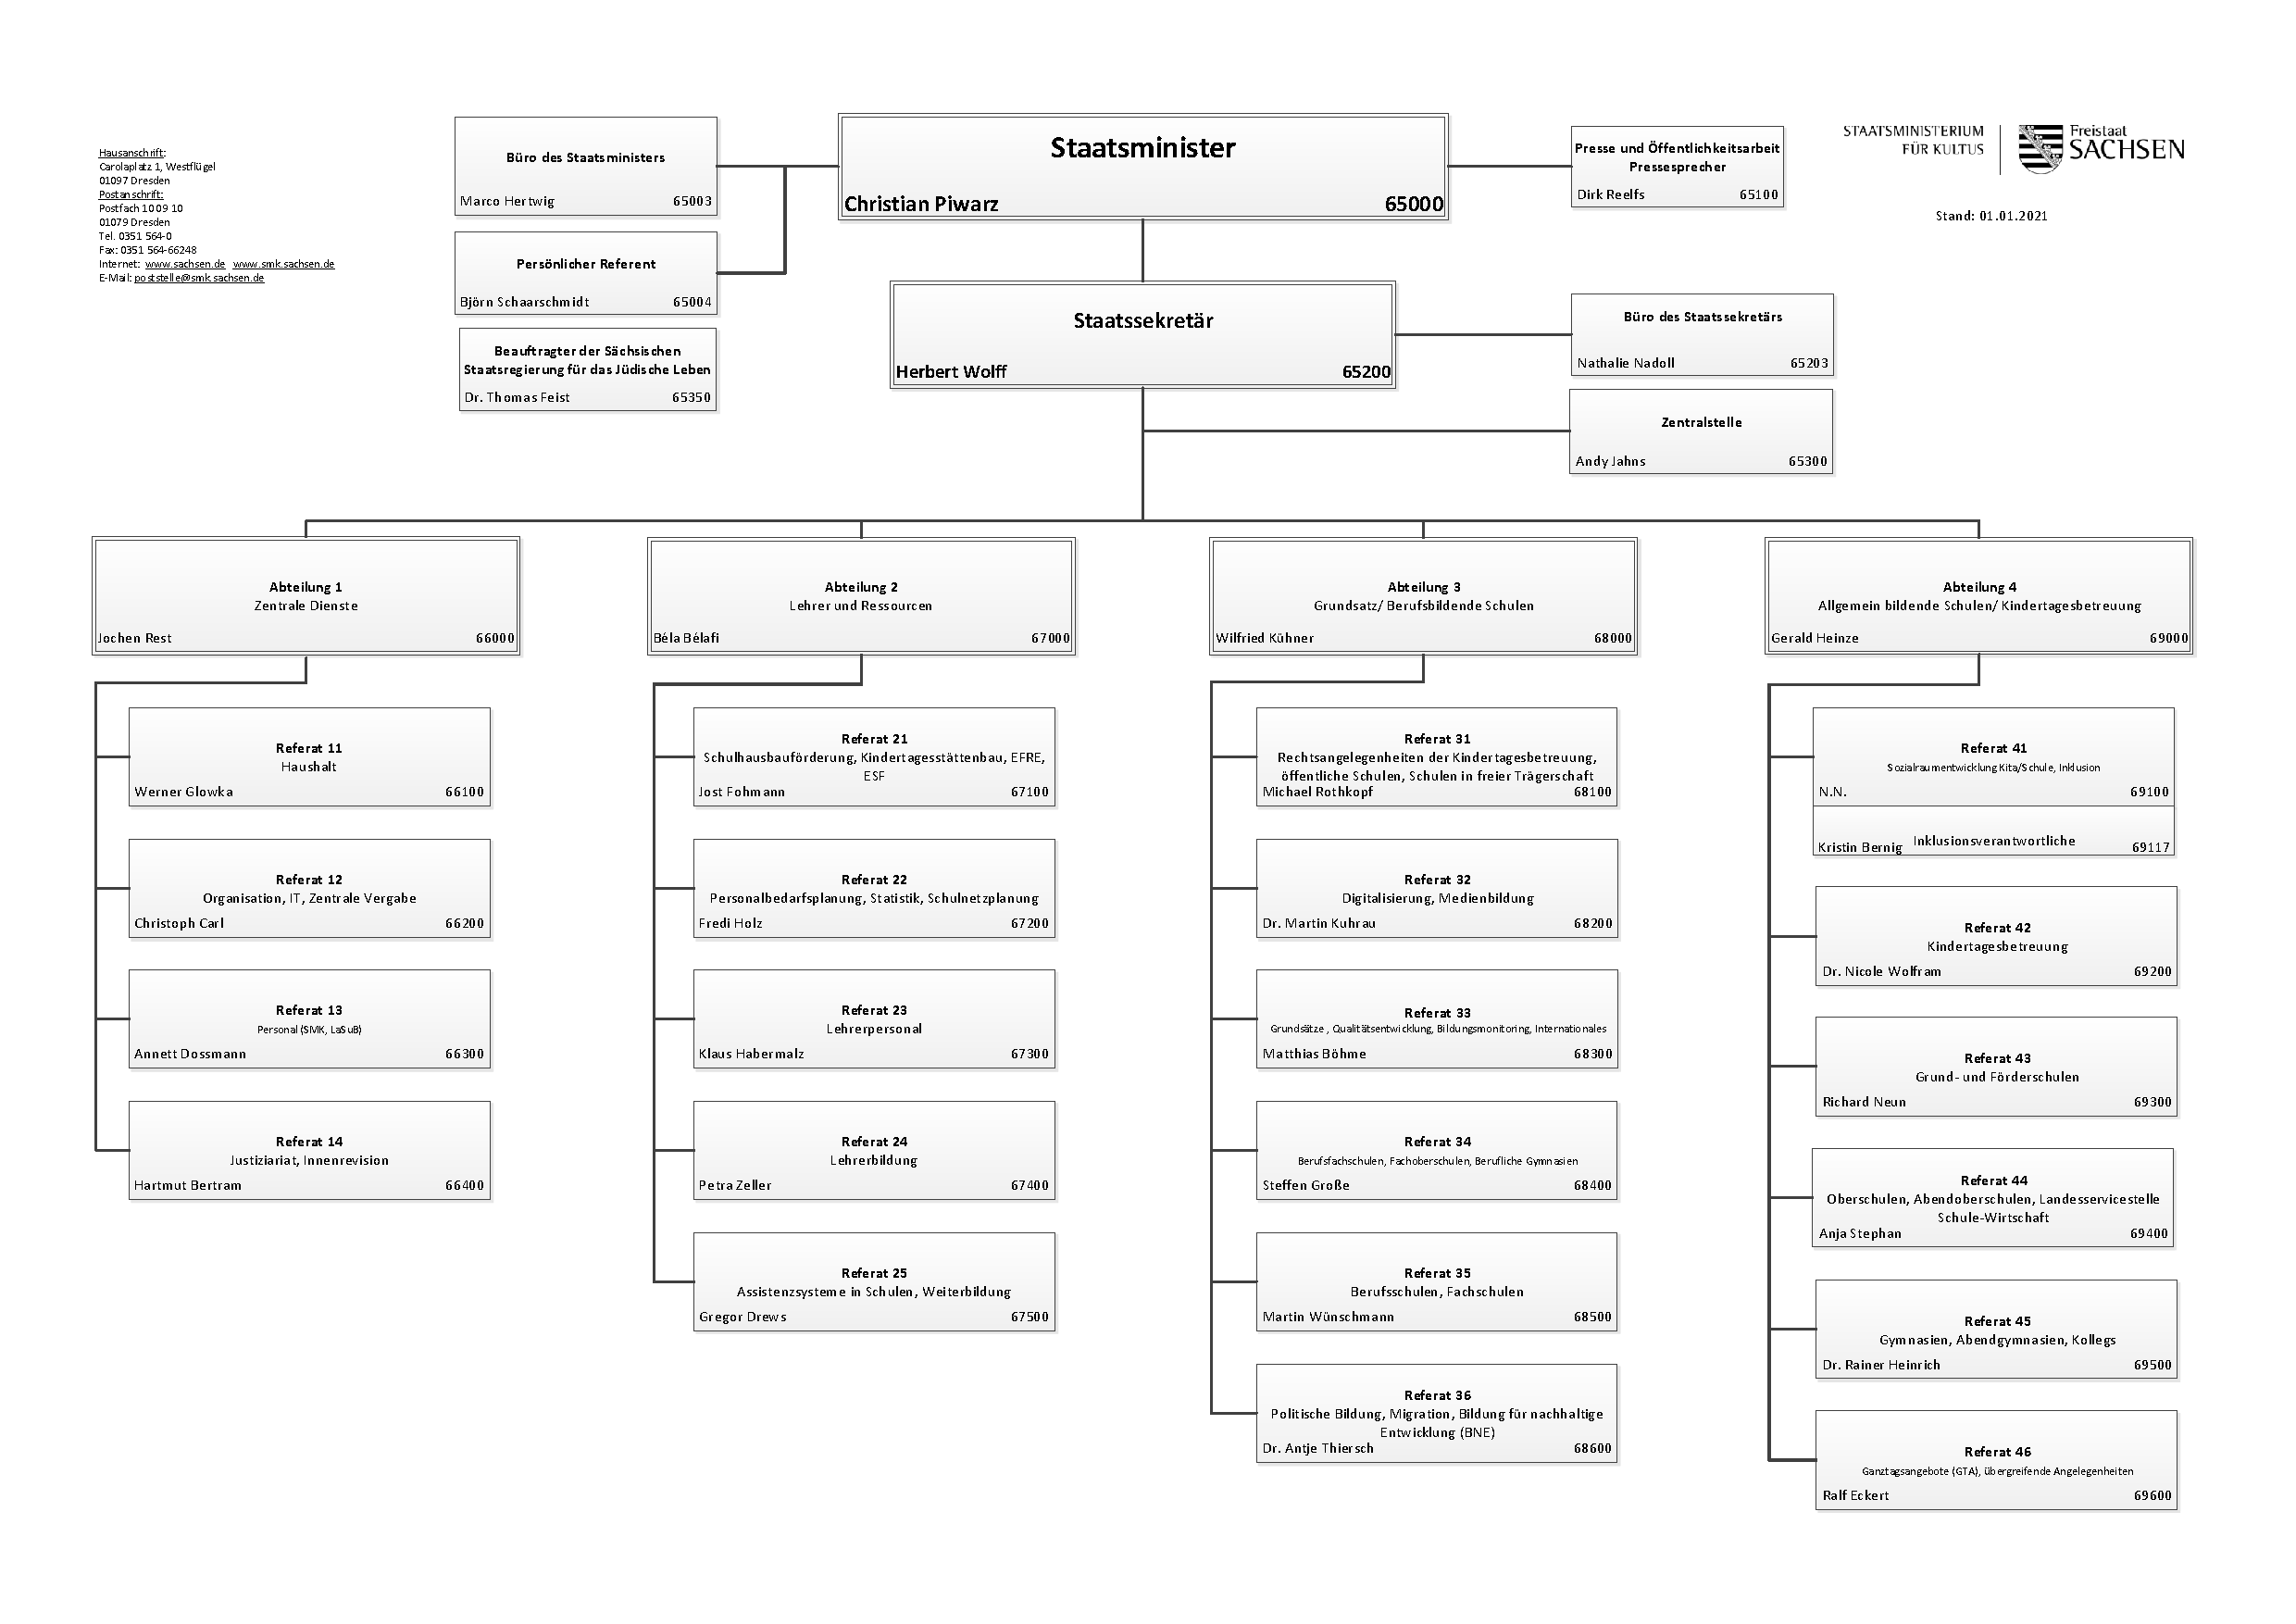
\includegraphics[angle=90, page=1,height=0.90\textheight, keepaspectratio]{anhang/abb/21_01_06_Organigramm_SMK.pdf}

\section{Gantt}
\label{abb:Gantt}
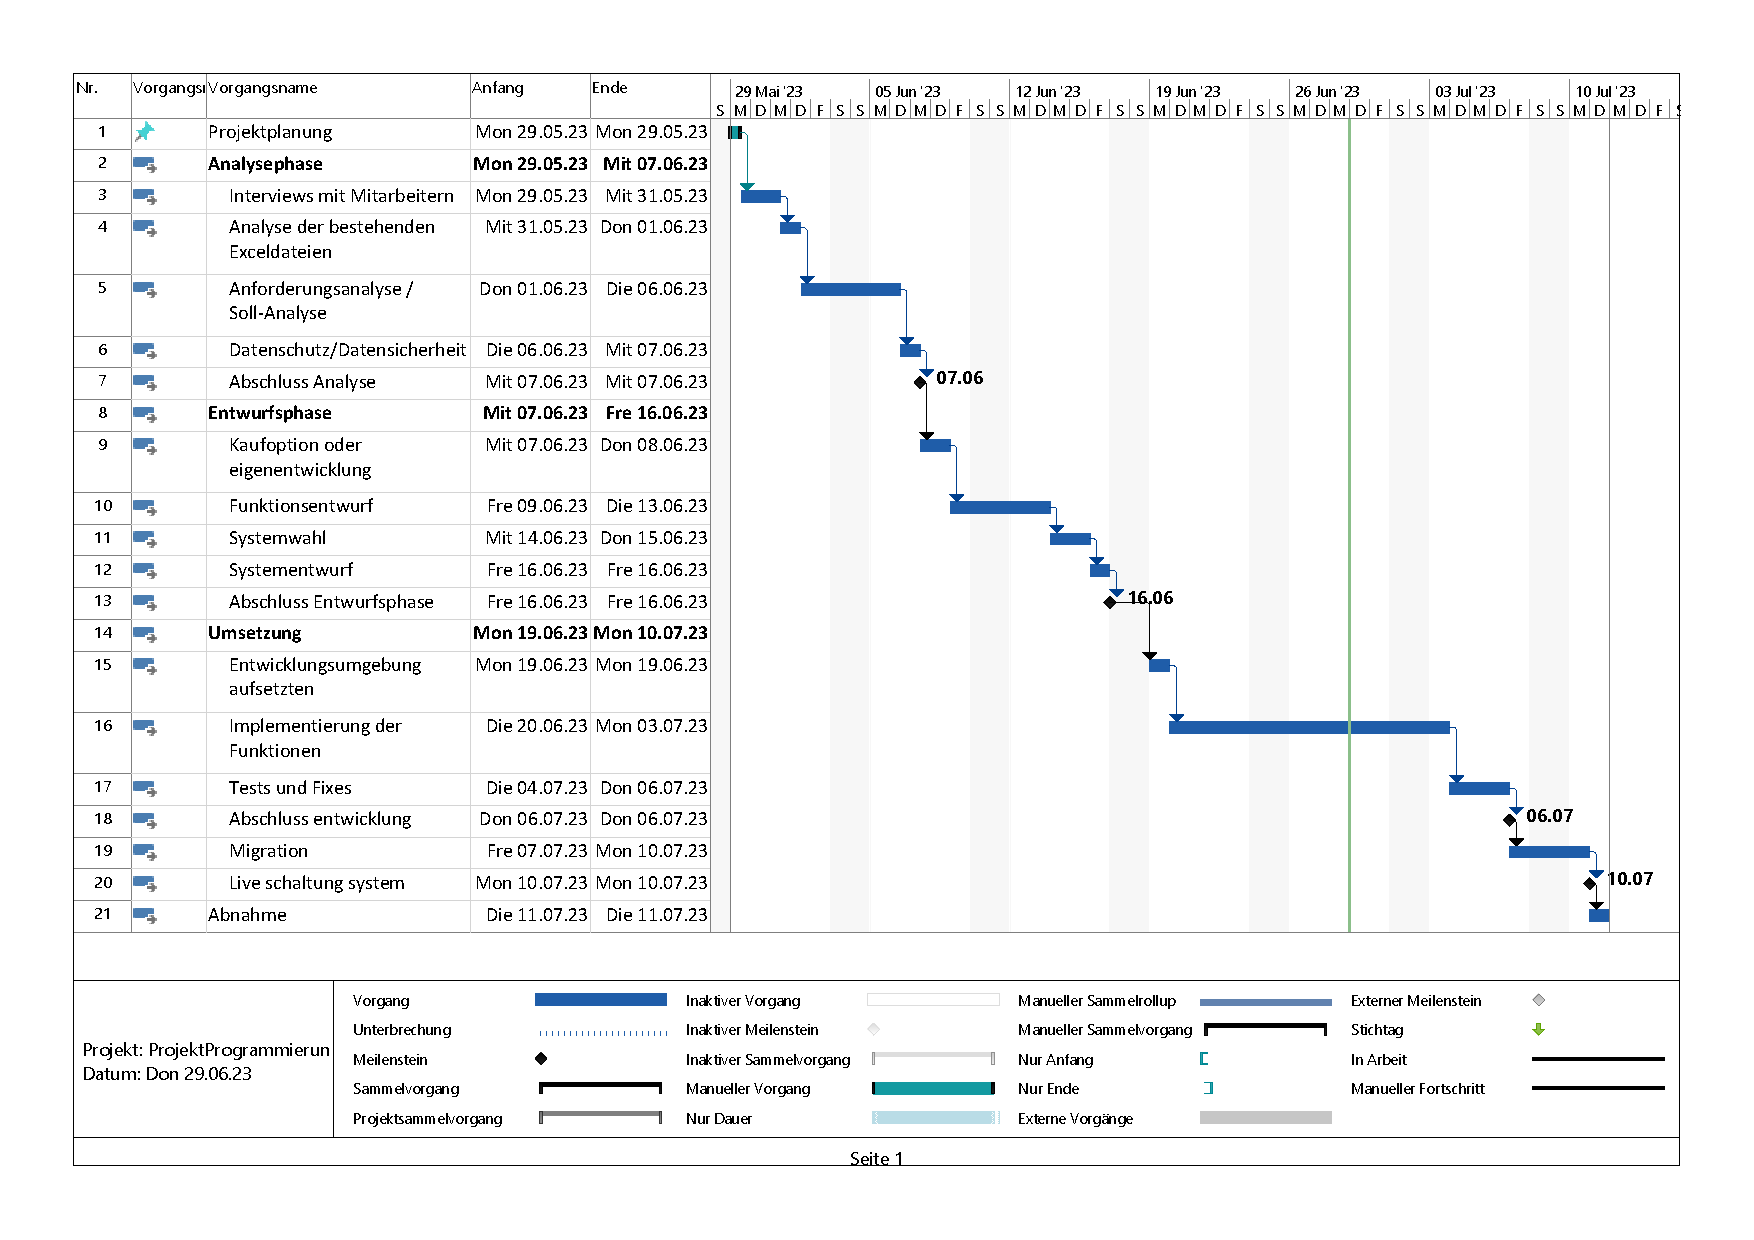
\includegraphics[angle=90, page=1,height=0.90\textheight, keepaspectratio]{anhang/abb/ProjektProgrammierungZeitplan.pdf}

\section{Ausgangstabelle}
\label{abb:Ausgangstabelle}
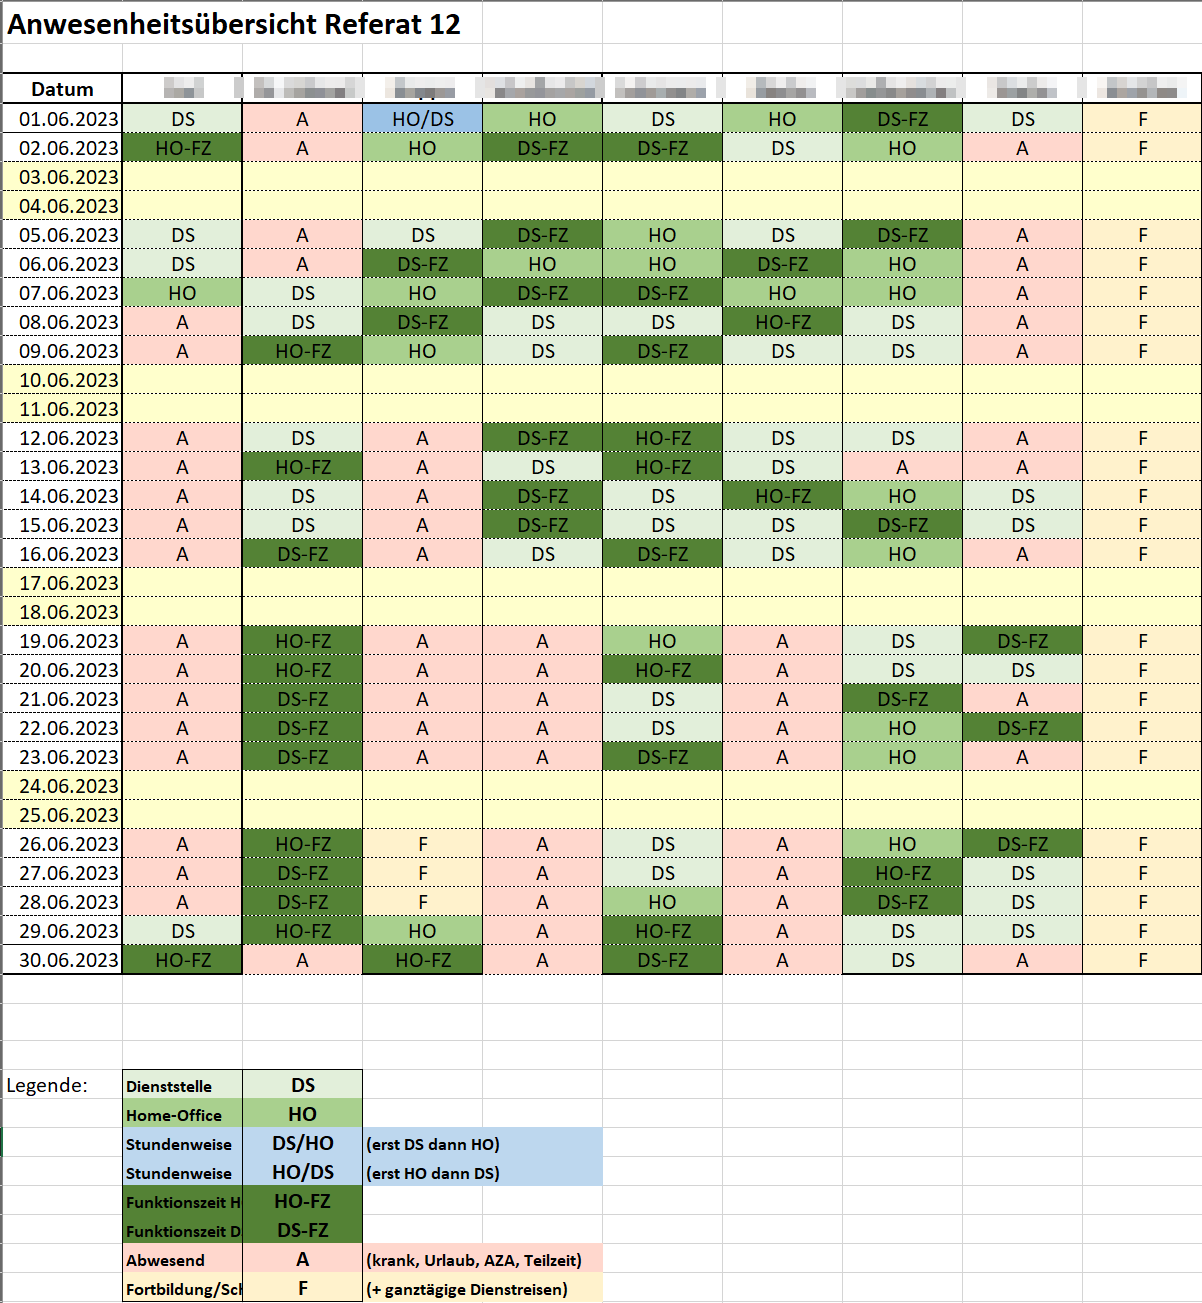
\includegraphics[page=1,height=1\textwidth]{anhang/abb/Tabelle.png}


\begin{figure}[htb]
    \centering
    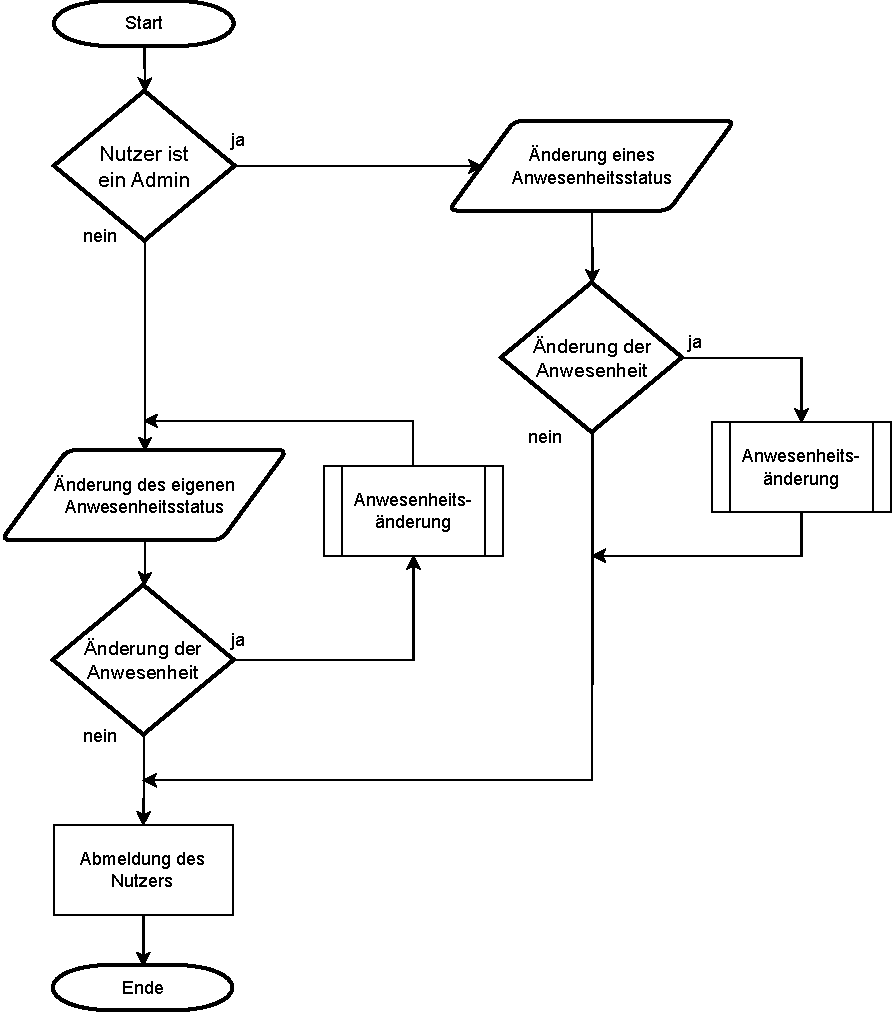
\includegraphics[width=0.9\textwidth,angle=0]{anhang/abb/PAP_Kurz.pdf}
    \caption[Beschreibung]{PAP änderungsvorgang von Anwesenheiten}
    \label{abb:PAP}
\end{figure}

\begin{figure}[htb]
    \centering
    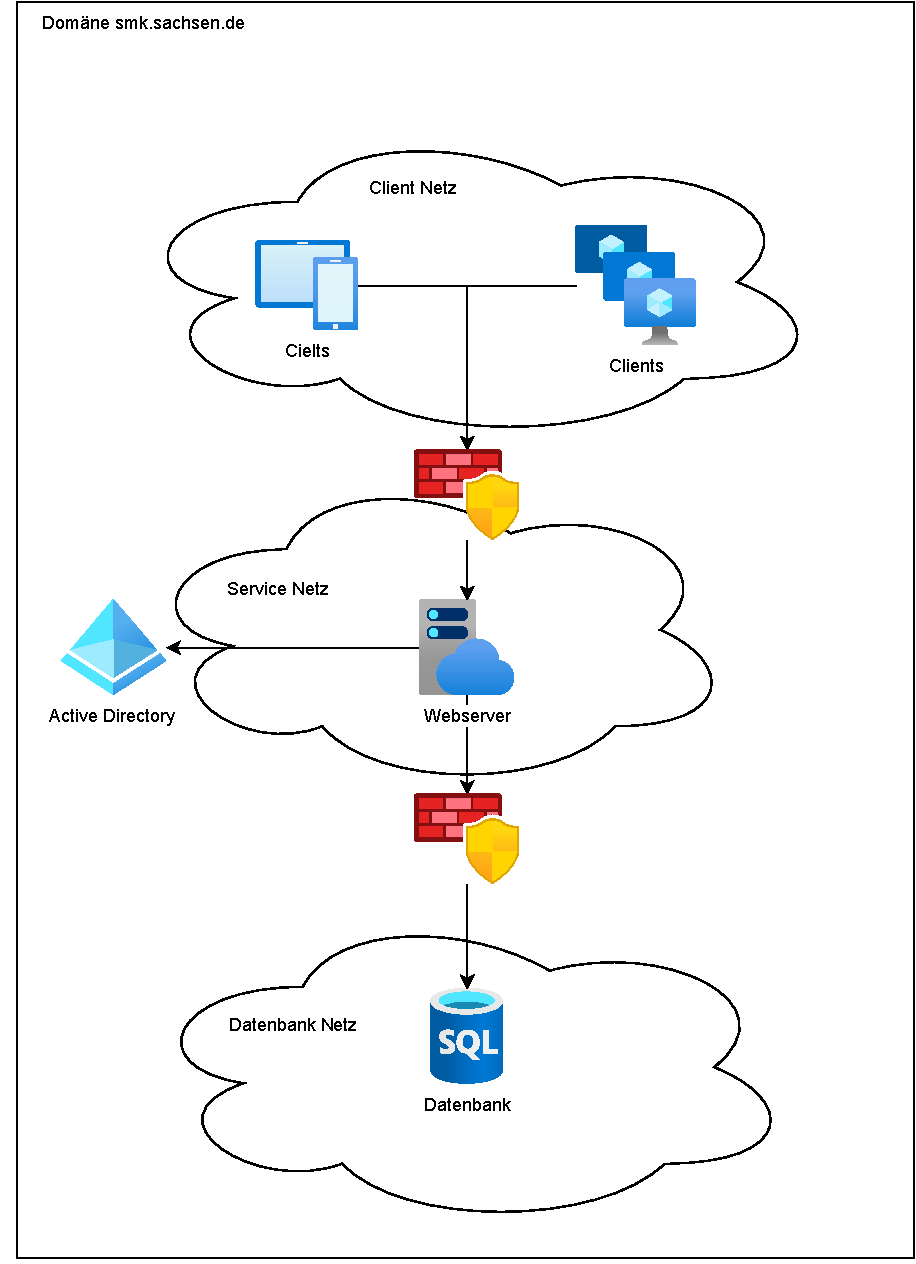
\includegraphics[width=0.9\textwidth,angle=0]{anhang/abb/Systemarchitektur.pdf}
    \caption[Beschreibung]{Systemarchitektur}
    \label{abb:Systemarchitektur}
\end{figure}


\end{document}
